\documentclass[reqno]{immbook}
%
\usepackage{amsmath}
\usepackage{amsfonts}
\usepackage{amssymb}
%
\usepackage{graphicx}
%\usepackage{makeidx}
%
%
\newcommand{\Real}{\mathbb{R}}
%
\newcommand{\BA}{\vec{\textbf{a}}}
\newcommand{\BB}{\vec{\textbf{b}}}
\newcommand{\BF}{\vec{\textbf{f}}}
\newcommand{\BG}{\vec{\textbf{g}}}
\newcommand{\BP}{\vec{\textbf{p}}}
\newcommand{\BQ}{\vec{\textbf{q}}}
\newcommand{\BU}{\vec{\textbf{u}}}
\newcommand{\BV}{\vec{\textbf{v}}}
\newcommand{\BW}{\vec{\textbf{w}}}
\newcommand{\BX}{\vec{\textbf{x}}}
\newcommand{\BY}{\vec{\textbf{y}}}
%
\newcommand{\BZ}{\vec{\textbf{0}}}  % Bold Zero (not "Z")
%
\newcommand{\T}{\rule{0pt}{2.6ex}}
\newcommand{\B}{\rule[-1.2ex]{0pt}{0pt}}
%
\newcommand{\ds}{\displaystyle}
%
\newtheorem{theorem}{Theorem}
%
\title{\textbf{Interdisciplinary Mathematical Modeling}}
\author{Warren Weckesser\\
Department of Mathematics\\
Colgate University}
%
\newtheorem{question}{Question}
%
\numberwithin{equation}{chapter}
%
\makeindex
%
\begin{document}
\frontmatter
\maketitle
\tableofcontents
%
%
%%%%%%%%%%%%%%%%%%%%%%%%%%%%%%%%%%%%%%%%%%%%%%%%%%%%%%%%%%%
%

\chapter*{Foreword}
\paragraph{Rough notes for now...}
\begin{itemize}
\item Goals: (i) Convert a description of a dynamical process
into a set of mathematical equations.
(ii) Use an appropriate combination of analysis and computer
simulation to study the mathematical model.
\item  I have intentionally minimized the
number of examples from physics.
One goal of this book is
to promote the use of mathematical models in fields outside of the
physical sciences.
\item The emphasis of the modeling is dynamic processes.
The mathematical topics are differential equations, discrete maps,
and Markov Chains (which are, in fact, linear maps).
Optimization, linear programming and other related topics
are \emph{not} covered in this book.
\item Prerequisite for the book include calculus (single variable)
and basic linear algebra.  The essential facts from linear algebra that
are needed in this book are summarized in an appendix.
\end{itemize}
%
\mainmatter
%
%
%%%%%%%%%%%%%%%%%%%%%%%%%%%%%%%%%%%%%%%%%%%%%%%%%%%%%%%%%%%
%

\chapter{Introduction}
%
%
%%%%%%%%%%%%%%%%%%%%%%%%%%%%%%%%%%%%%%%%%%%%%%%%%%%%%%%%%%%
%

\chapter{Differential Equations}

\section{Modeling with Differential Equations}
\emph{Start with an example; discuss significance of a
relationship between and function and its derivative...}
%
The general form of a first order (autonomous) differential
equation is
\[
   \frac{dy}{dt} = f(y)
\]
\noindent
If  $f'(y_{0})=0$, then $y(t)=y_{0}$ is a solution.  Such a constant
solution is called an \emph{equilibrium solution}.\index{equilibrium}

\section{Unconstrained Population Growth}


The simplest assumption for modeling the growth of a population
is:
\begin{quote}
\emph{The rate of change of the population is proportional to the current population level.}
\end{quote} 
Let $t$ be time, and let $p(t)$ be the population at time $t$.
For now we'll assume that some convenient system of units is used;
we'll have more to say about units later.
We also assume that $p$ is ``large'' in some sense, so that it is reasonable
to treat $p$ as a real number, not an integer.  If, for example, the population
was just three rabbits, the following models would probably not provide good
approximations to the actual growth of the population.  If the population
is measured in thousands of rabbits, then $p(0)=3.12$ makes sense,
and the following models are more reasonable.

We convert the above assumption into an equation involving $t$
and $p$.
The ``rate of change of the population'' is the derivative, $\frac{dp}{dt}$, and the
current population is $p(t)$, so the mathematical version of the above
assumption is
\begin{equation}
  \frac{dp}{dt} = rp
\end{equation}
where $r$ is the constant of proportionality.
(Note that I have suppressed the argument of $p$ for brevity.)
This is a \emph{first order differential equation}.
(The \emph{order} of a differential equation is the order of the
highest derivative in the equation.)

Frequently, the question we ask is ``What is the population at time $t$
if the population is $P_0$ at time $t=0$?''  That is, we impose the
condition that $p(0)=P_0$.  This is called an
\emph{initial condition}, and the problem of solving the differential
equation with a given initial condition is called an
\emph{initial value problem}.

To solve this equation, we must find a \emph{function} $p(t)$
that satisfies the equation.  In this case, the solution is
\begin{equation}
  p(t) = P_0 e^{rt}
\end{equation}
(Let's check:  $\frac{dp}{dt} = rP_0e^{rt} = r p(t)$, so  it solves the differential
equation, and $p(0) = P_0e^0 = P_0$, so it also satisfies the initial condition.)
Thus, if $r > 0$, the simple assumption given above results in
\emph{exponential growth}.\index{exponential growth}
(If $r < 0$, we obtain \emph{exponential decay}.\index{exponential decay})

\section{The Logistic Equation\index{logistic equation}}

For a population with unlimited resources, exponential growth
is a pretty accurate description of what happens.
However, no environment can support exponential growth forever.
Eventually the food runs out, or there is simply not enough space
for a larger population.
Presumably there is a maximum population level that the environment
can sustain.  This level is called the
\emph{carrying capacity}\index{carrying capacity}
of the environment. If the population is larger than the
carrying capacity, overcrowding or a lack of food results in a
\emph{decreasing} population.
We'll modify the equation to take this into account.

The right side of the equation gives the rate of change of $p$ as a function
of $p$.
If we divide the the right side by $p$, we obtain the
\emph{per capita growth rate},
or simply the \emph{growth rate}.\index{growth rate}
For the initial assumption,
the growth rate  is just the constant $r$.
To incorporate the assumption of a carrying capacity, we will assume that the
growth rate depends on $p$.  When $p$ is near zero, we assume that there
are plenty of resources for the population to grow, so the growth rate should be
near $r$.  As the population becomes bigger, the growth rate should decrease,
and it should be zero when the population is at the carrying capacity.
If the population exceeds the carrying capacity, the growth rate should
be negative.

The simplest formula for such a growth rate is a straight line that has
the value $r$ when $p=0$ and the value $0$ when $p=K$, as shown in
Figure~\ref{fig:growthrate}.
\begin{figure}
\centerline{\includegraphics[width=3in]{matlab/logistic_percapita_growthrate.eps}} 
\caption{Per capita growth rate for the logistic equation.}
\label{fig:growthrate}
\end{figure} 
The equation that we obtain is
\begin{equation}
  \frac{dp}{dt} = r\left(1-\frac{p}{K}\right)p
\label{eqn:logistic}
\end{equation}
This first order differential equation is commonly called the \emph{logistic equation}.\index{logistic equation}
Later we'll see how to find the exact solutions to this equation.
For now, we'll learn as much as we can about its solutions without actually solving the
equation.  To do this, we plot the right side of \eqref{eqn:logistic} as a function of $p$.
The graph is shown in Figure~\ref{fig:logisticrhs}.
\begin{figure}
\centerline{\includegraphics[width=3in]{matlab/logistic_growthrate.eps}} 
\caption{A plot of $\frac{dp}{dt}$ as a function of $p$ for the logistic
equation \eqref{eqn:logistic}.}
\label{fig:logisticrhs}
\end{figure}
We can use the information in Figure~\ref{fig:logisticrhs} to determine the
behavior of solutions to \eqref{eqn:logistic}.
Suppose, for example, that the population is initially ``small''.
(In this case, small means ``a small fraction of $K$''.)
Then the graph in Figure~\ref{fig:logisticrhs} tells us that
$\frac{dp}{dt}$ is also small but positive.  In other words, the slope
of $p(t)$ is small and positive.  This means that $p(t)$ is an increasing
function of $t$, so in a little while, $p$ will be larger.  Looking back to
Figure~\ref{fig:logisticrhs}, we see that this means $\frac{dp}{dt}$ will be
larger than it was before, and therefore the slope of $p(t)$ has increased.
So initially, $p(t)$ will grow faster and faster.  This is not surprising, since
when $p$ is small, $p^2$ is very small, and if we ignore the $p^2$ term in the
logistic equation, we obtain $\frac{dp}{dt} \approx rp$.  So when the
population is small, the growth is almost exponential.

Eventually the population will reach $K/2$.  This is the population
level at which the population grows the fastest.
When the population reaches this level, further increases in the
population result in \emph{lower} growth rates.
For example, if $p(t) = 0.75K$ at some time $t$, we see in
Figure~\ref{fig:logisticrhs} that $\frac{dp}{dt}$ is positive, but it is
decreasing as $p$ increases.  In the next moment, $p$ will be larger,
but then the slope of $p(t)$ will be smaller.
As $p$ gets closer and closer to $K$, the slope gets smaller and smaller.
In fact, $p(t)$ will approach $K$ asymptotically, but never reach it.
A graph of a solution to the logistic equation~\eqref{eqn:logistic} is
shown in Figure~\ref{fig:logisticsol}.
\begin{figure}
\centerline{\includegraphics[width=3in]{matlab/logistic_solution.eps}} 
\caption{The graph of $p(t)$, a solution to the logistic
equation \eqref{eqn:logistic}.}
\label{fig:logisticsol}
\end{figure}

\begin{question}
Describe (and sketch) the solution that
results when the initial population is greater than $K$.
\end{question}

Note that if the initial population is exactly $K$, then
$\frac{dp}{dt} = 0$.  The constant function $p(t)=K$ is an
exact solution to the differential equation.
We call a constant solution an
\emph{equilibrium solution}.\index{equilibrium solution}

\begin{question}
Does the logistic equation \eqref{eqn:logistic} have any other
equilibrium solutions?
\end{question}

The method for analyzing solutions to the logistic equation can be
applied to any first order equation of the form
\begin{equation}
   \frac{dy}{dt} = f(y)
\end{equation}
where $f(y)$ is a given function.
In particular, we assume that $t$ does \emph{not} appear explicitly
in $f$.  Such an equation is called \emph{autonomous}.\index{autonomous}
When $t$ appears explicitly in the right side of the equation,
we say the equation is \emph{nonautonomous}.\index{nonautonomous}
For example, the equation
\begin{equation}
  \frac{dp}{dt} = (r+a \sin(\omega t))p
\end{equation}
is nonautonomous, since $t$ appears explicitly in the right side of the
equation (in the argument of the sine function).
In this case, the explicit time dependence might model a growth
rate with seasonal dependence.

The basic procedure to analyze an autonomous
first order differential equation is to sketch the graph of $f(y)$, identify
the equilibrium solutions (where $f(y)=0$), and determine the
behavior of non-equilibrium solutions based on the graph
of $f(y)$.

\begin{question}
Consider the differential equation
\[
   \frac{dy}{dt} = y(y-1)(y-2)
\]
(a) Find the equilibrium solutions.\\
(b) Sketch $\frac{dy}{dt}$ as a function of $y$.\\
(c) In one set of axes, sketch several solutions $y(t)$. Include the equilibrium solutions,
and several more non-equilibrium solutions to show all the possible behaviors.
(Since this is not necessarily a population model, you should consider negative values
of $y$ as well as positive.)
\end{question}



\section{Separable First Order Differential Equations (*)}

In this section and the next, we discuss
two techniques for solving certain first order
differential equations.
The general form for a first order differential equation is
\begin{equation}
   y'(t) = f(t,y)
\end{equation}
In this section we discuss \emph{separable} equations,
and in the next we discuss \emph{linear} equations.

\medskip
If $f$ can be ``separated'' into a quotient of a function of $t$ and a function
of $y$ as
\begin{equation}
   f(t,y) = \frac{h(t)}{g(y)},
\end{equation}
there is a chance that the solutions can
be found analytically.
The differential equation may be written
\begin{equation}
  g(y(t))y'(t) = h(t)
\label{eqn:separated}
\end{equation}
We now integrate both sides:
\begin{equation}
    \int_0^t g(y(s))y'(s) \, ds = \int_0^t h(s) \, ds
\label{eqn:integrated}
\end{equation}
The right side is an integral of a known function.
To deal with the left side, we first let $p(y) = \int_{y_0}^y g(z) dz$.
Then  we use the chain rule:
\begin{equation}
   \frac{d}{dt} p(y(t)) = p'(y)y'(t) = g(y)y'(t).
\end{equation}
Thus, on the left side of \eqref{eqn:integrated}, we have
\begin{equation}
  \int_0^t g(y)y'(s)\,ds = \int_0^t \left(\frac{d}{ds} p(y(s))\right)\, ds = p(y(t)) = 
    \int_{y_0}^y g(z) \, dz
\end{equation}
The net result can be summarized with the following formal procedure:
\begin{enumerate}
\item Treat the derivative $\frac{dy}{dt}$ as a fraction and rewrite the differential equation
as
\begin{equation}
   g(y)dy = h(t)dt.
\end{equation}
\item Integrate with respect to $y$ on the left and with respect to $t$ on the right.
The constants of integration can be combined into one constant on the right after
integrating.
\item Solve for $y$.
\end{enumerate}
The \emph{real} short summary is:
\begin{quote}
  \emph{Separate}, \emph{Integrate}, \emph{Isolate} (i.e. solve for $y$).
\end{quote}
Note that even if $f$ can be separated into $h(t)/g(y)$, there are two potential obstacles
to this method. First, it might not be possible to evaluate the integrals.
Second, it might not be possible to solve for $y$ after integrating.
In this case, we have an implicit equation relating $y$ and $t$, which can still
be useful in some cases.

Note that all autonomous first order differential equations are separable.

\paragraph{Example 1.}
We'll apply the method to
\begin{equation}
   \frac{dp}{dt} = r p
\end{equation}
In this case, separating gives
\begin{equation}
   \frac{dp}{p} = r dt,
\end{equation}
but note that we have assumed that $p\ne 0$.
Integrating gives
\begin{equation}
   \ln | p | = rt+C_0
\end{equation}
Exponentiate both sides to obtain
\begin{equation}
  |p| = e^{rt+C_0} = C_1e^{rt}, \quad \textrm{where} \quad C_1 = e^{C_0}.
\end{equation}
Note that $C_1 > 0$.
For $p > 0$, we have $|p|=p$, so $p=C_1e^{rt}$.
If $p < 0$, $|p| = -p$, so $p = -C_1e^{rt}$.
This is the same as saying the constant in front of $e^{rt}$ is negative.
Also note that $p(t)=0$ is an equilibrium solution.
We can combine the three cases $p>0$, $p=0$ and $p<0$ into one
solution
\begin{equation}
   p(t) = Ce^{rt},
\end{equation}
where $C$ is an arbitrary constant.
To satisfy an initial condition $p(0)=P_0$, we let $C=P_0$.

\paragraph{Example 2.}
Now consider a population model in which the per capita growth
rate varies periodically.  This might be because of seasonal variation.
The differential equation is
\begin{equation}
   \frac{dp}{dt} = (r + a\cos(\omega t))p
\end{equation}
Separating gives
\begin{equation}
  \frac{dp}{p} = \left( r+a\cos(\omega t) \right) dt
\end{equation}
and integrating gives
\begin{equation}
  \ln | p | = rt + \frac{a}{\omega} \sin(\omega t) + C_0
\end{equation}
From here, the work is similar to the previous example.
The final concise formula for the solution is
\begin{equation}
   p(t) = Ce^{rt + (a/\omega)\sin(\omega t)}
\end{equation}
where $C$ is an arbitrary constant.
%
%
\section{Linear First Order Differential Equations (*)}

If the first order differential equation has the form
\begin{equation}
    y'(t) = p(t) y + g(t),
\label{eqn:linear}
\end{equation}
it is called a \emph{linear} equation.
We can always express the solution to such an equation
in terms of integrals.  The only obstacle will be
evaluating the integrals.

To derive the solution, we first simply move $p(t)y$ to the left:
\begin{equation}
    y'(t) - p(t) y =  g(t),
\label{eqn:intermediateA}
\end{equation}
The left side looks vaguely like the result of applying the
product rule of differentiation to a product of $y$ and something else.
If $\mu(t)$ is some function, then $(\mu y)' = \mu y' + \mu' y$,
which suggests that we multiply \eqref{eqn:intermediateA}
by $\mu$ (whatever it is)
to obtain
\begin{equation}
    \mu y'(t) - \mu p(t) y =  \mu g(t),
\label{eqn:intermediateB}
\end{equation}
and then determine what $\mu(t)$ should
be by solving $\mu' = -\mu p(t)$.
This is a separable equation; a solution is
\begin{equation}
   \mu(t) = e^{-\int p(t)\, dt}.
\end{equation}
We could include an arbitrary multiple of this function
by multiplying it by an arbitraryconstant $C$, but we
don't need it.  Equivalently, when we find the integral
$\int p(t)\,dt$, we may choose the constant of integration
to be zero.

With this choice of $\mu$, 
\eqref{eqn:intermediateB} becomes
\begin{equation}
    (\mu y)' =  \mu g(t).
\label{eqn:intermediateC}
\end{equation}
Integrating both sides gives%
\footnote{Note that I have explicitly included the integration
constant $C$ on the right.  Normally, when we write an indefinite
integral $\int q(t)\, dt$, the constant of integration is implicitly
assumed to be part of the result. For example, $\int 2x\,dx = x^2+C$.
However, it is a common mistake to \emph{forget} the constant, so
I choose to include it explicitly.}
\begin{equation}
    \mu y =  \int \mu g(t) \, dt + C
\label{eqn:intermediateD}
\end{equation}
and so we have the following solution
to \eqref{eqn:linear}:
\begin{equation}
    y =  \frac{1}{\mu}\left(\int \mu g(t) \, dt + C\right)
    \quad \textrm{where} \quad
    \mu(t) = e^{-\int p(t)\, dt}.
\label{eqn:linearsolution}
\end{equation}

\paragraph{Example 1.}
Consider the initial value problem
\begin{equation}
   y' = 2y + 3, \quad y(0) = 5.
\label{eqn:linearexample1}
\end{equation}
This problem is linear, with $p(t)=2$ and $g(t) = 3$.
(It is also separable, so there is more than one way
to solve this problem.)
The integrating factor is
\begin{equation}
   \mu(t) = e^{-\int p(t)\,dt} = e^{-\int 2\, dt}
      = e^{-2t},
\end{equation}
and the solution is
\begin{equation}
\begin{split}
   y(t) & = e^{2t} \left( \int \left(e^{-2t}\right)\left(3\right)\,dt + C\right) \\
        & = e^{2t} \left( -\frac{3}{2} e^{-2t} +C \right) \\
	& = -\frac{3}{2} + Ce^{2t}.
\end{split}
\end{equation}
To satisfy the initial condition $y(0)=5$, we have
\begin{equation}
   y(0) = -\frac{3}{2} + C = 5 \implies C = \frac{13}{2} .
\end{equation}
So the solution to the initial value problem is
\begin{equation}
   y(t) = -\frac{3}{2} + \frac{13}{2}e^{2t}.
\end{equation}
You should check the answer by substituting it back
into \eqref{eqn:linearexample1}.

\paragraph{Example 2.}
\begin{equation}
   y' = -\frac{y}{t} + t, \quad y(1) = 2.
\end{equation}
In this case, $p(t) = -1/t$ and $g(t) = t$.
Note that the initial condition is given at
$t=1$ rather than the usual $t=0$.  Nothing
is wrong or difficult about that. We just have
to remember to evaluate the solution at $t=1$
when we solve for the constant to make
the solution satisfy the initial condition.
Also, since we can not divide by zero, we will
assume that we are only interested in the solution
where $t > 0$.

The integrating factor is
\begin{equation}
   \mu(t) = e^{-\int p(t)\,dt} = e^{\int \frac{1}{t}\, dt}
      = e^{\ln |t|} = e^{\ln t} = t,
\end{equation}
where, because we assume $t>0$,  we used $|t|=t$.
The solution is
\begin{equation}
\begin{split}
   y(t) & = \frac{1}{\mu} \left( \int \mu g(t)\,dt + C\right) \\
        & = \frac{1}{t} \left( \int t^2 \,dt+C\right) \\
	& = \frac{1}{t} \left( \frac{t^3}{3} + C \right)\\
	& = \frac{t^2}{3} + \frac{C}{t}
\end{split}
\end{equation}
To satisfy the initial condition $y(1)=2$, we have
\begin{equation}
   y(1) = \frac{1}{3} + C = 2 \implies C = \frac{5}{3}.
\end{equation}
Thus the solution to the initial value problem is
\begin{equation}
   y(t) = \frac{t^2}{3} + \frac{5}{3t}.
\end{equation}


\paragraph{Example 3.}
Consider the differential equation
\begin{equation}
    y' = 2ty + 3.
\end{equation}
The differential equation is linear, with p(t) = 2t and g(t)=3.
The integrating factor is
\begin{equation}
   \mu(t) = e^{-\int p(t)\,dt} = e^{-\int 2t\, dt}
      = e^{-t^2},
\end{equation}
and the solution is
\begin{equation}
\begin{split}
   y(t) & = e^{t^2} \left( \int \left(e^{-t^2}\right)\left(3\right)\,dt + C\right) \\
        & = e^{t^2} \left( 3\int e^{-t^2}\,dt+C\right)
\end{split}
\end{equation}
There is no analytical expression for the integral $\int e^{-t^2}\, dt$,
so this is the best we can do.%
\footnote{%
Because the integral of $e^{-t^2}$ appears frequently in mathematics,
it has been given a name.
You may have seen the \emph{error function}
$\textrm{erf}(x) = \frac{2}{\sqrt{\pi}}\int_0^x e^{-s^2}\,ds$.}


\subsection*{Exercises}
\begin{enumerate}
\item For each of the following differential equations,
determine the equilibrium solutions, sketch $f(y)$ as a function
of $y$, and sketch the solutions where $y(0)=1/2$, $y(0)=1$, and
$y(0)=3/2$.
\begin{enumerate}
\item $\ds y' = -2y + 1$
\item $\ds y' = y(2-y)$
\item $\ds y' = \sin(\pi y)$
\end{enumerate}
\item
If possible, find a formula for the solutions to the
differential equations in Exercise 1.
\item
\emph{...a question in which a description must be converted to
a differential equation...}
\item
\emph{...another...}
\end{enumerate}

\section{Systems of Differential Equations}

A general form for a \emph{system} of $n$ first order differential
equations is
\begin{equation}
\begin{split}
  \frac{dx_1}{dt} & = f_1(t,x_1,x_2,\ldots,x_n) \\
  \frac{dx_2}{dt} & = f_2(t,x_1,x_2,\ldots,x_n) \\
  \vdots \\
  \frac{dx_n}{dt} & = f_n(t,x_1,x_2,\ldots,x_n)
\end{split}
\end{equation}
If all the functions $f_i$ on the right do not explicitly depend on
$t$, we say the system is \emph{autonomous};\index{autonomous} otherwise it is
\emph{nonautonomous}.\index{nonautonomous}
We may write the system in vector notation as
\begin{equation}
   \frac{d\BX}{dt} = \BF(t,\BX),
      \quad
      \textrm{where}
      \quad
      \BX(t) = \begin{bmatrix} x_1(t) \\ x_2(t) \\ \vdots \\ x_n(t)\end{bmatrix}
      \quad
      \textrm{and}
      \quad
      \BF(t,\BX) = \begin{bmatrix} f_1(t,\BX) \\ f_2(t,\BX) \\ \vdots \\ f_n(t,\BX) \end{bmatrix}
\end{equation}
We will focus on the autonomous system
\begin{equation}
   \frac{d\BX}{dt} = \BF(\BX).
\end{equation}
The function $\BF$ is called a \emph{vector field}.
It assigns a vector to each point in $\mathbb{R}^n$.
The vector function $\BX(t)$ is a curve in $\mathbb{R}^n$,
parameterized by $t$.
(In this context, $\mathbb{R}^n$ is often called
the $\emph{phase space}$.)
The derivative $\frac{d\BX}{dt}$ is a vector tangent to
the curve.
If we interpret $\BX(t)$ as the motion of a particle
in $\mathbb{R}^n$, then $\frac{d\BX}{dt}$ is the \emph{velocity}
of the particle.
\emph{Solving} the differential equation means finding
the vector function
$\BX(t)$ such that its velocity matches the given vector field
at all points along the curve.

\paragraph{The Phase Plane.}\index{phase plane}
In the two dimensional autonomous case, the phase space
is called the \emph{phase plane}.
The system of equations can be rewritten as
\begin{equation}
\begin{split}
    \frac{dx}{dt} & = f(x,y) \\
    \frac{dy}{dt} & = g(x,y)
\end{split}
\end{equation}
\paragraph{Example: The SI Components of the SIR Model.}
We have previously seen the SIR model of the spread of
a disease in a population:
\begin{equation}
\begin{split}
   \frac{dS}{dt} & = -rSI \\
   \frac{dI}{dt} & = rSI -\gamma I \\
   \frac{dR}{dt} & = \gamma I
\end{split}
\end{equation}
Note that the first two equations do not depend on $R$.
We can analyze the first two equations as a two dimensional
system, and then infer the values of $R$ from the
relation $S+I+R=N$, where $N$ is the (constant) size
of the total population.

We state without proof the following theorems.
\begin{theorem}
Uniqueness...
\end{theorem}
This theorem means that trajectories in phase
space do not cross each other.
\section{Phase Plane Analysis\index{phase plane}}

The system of differential equations is
\begin{equation}
\begin{split}
   \frac{dx}{dt} & = f(x,y) \\
   \frac{dy}{dt} & = g(x,y)
\end{split}
\end{equation}
or
\begin{equation}
  \frac{d\BX}{dt} = \BF(\BX), \quad \BX \in \mathbb{R}^2, \quad
      \BF : \mathbb{R}^2 \rightarrow \mathbb{R}^2.
\end{equation}

The basic steps are
\begin{enumerate}
\item Find the equilibrium solutions.
This means we must solve simultaneously
\begin{equation}
    f(x,y) = 0 \quad \textrm{and} \quad g(x,y) =0.
\end{equation}
(This may turn out to be very hard or impossible!)
\item Find and sketch the $x$ and $y$ \emph{nullclines}.

The $x$ nullclines are the curves where $\frac{dx}{dt}=0$, which
is the set of points where $f(x,y)=0$.
Since the $x$ component of the vector field is zero on the
$x$ nullcline, trajectories cross the $x$ nullcline with
vertical tangents.

Similarly, the $y$ nullclines are the curves where
$\frac{dy}{dt} = 0$, which is the set of points where $g(x,y) = 0$.
Trajectories cross the $y$ nullclines with horizontal tangents.

Note that each intersection of an $x$ nullcline and a $y$ nullcline
is an equilibrium.

Once the nullclines are sketched, figure out the direction of the
vector field on each nullcline. To do this, simply pick a few points
on the nullclines and plug them into $\BF(\BX)$.

\item
The nullclines divide the phase plane in regions.  In each
region, $\frac{dx}{dt}$ and $\frac{dy}{dt}$ have constant sign.
This lets us determine (very roughly!) the direction of the
vector field for all points in each region.  For example,
if $\frac{dx}{dt} > 0$ and $\frac{dy}{dt} < 0$ in some region,
then all vectors in the vector field are pointing
``down and to the right'' (i.e. negative $y$ direction,
positive $x$ direction).
\end{enumerate}
The above steps are often enough to obtain a
pretty good idea of the behavior of the trajectories
in the phase plane.


\section{Planar Linear Systems}


We consider the linear system of two first order
differential equations
\begin{equation}
\begin{split}
  \frac{dx}{dt} & = ax + by \\
  \frac{dy}{dt} & = cx + dy
\end{split}
\end{equation}
or equivalently,
\begin{equation}
  \frac{d\BX}{dt} = A\BX, \quad \textrm{where} \quad
     \BX = \begin{bmatrix} x \\ y \end{bmatrix},
     \quad \textrm{and} \quad
     A = \begin{bmatrix} a & b \\ c & d \end{bmatrix}.
\label{eqn:linearsys}
\end{equation}

\subsection*{Solving the System}
To solve this system, we first recall that the solution to the
single equation
\begin{equation}
  \frac{dx}{dt} = a x
\end{equation}
is $x(t) = c e^{at}$: a constant multiplied by
an exponential.  We also recall that the last problem of Homework 2
was a linear system, and the solution to that problem can be
written in vector form as
\begin{equation}
 \BX(t) = \begin{bmatrix} \frac{y_0}{2} \\ y_0 \end{bmatrix} e^{-t}
            +\begin{bmatrix} -\frac{y_0}{2}+x_0 \\ 0 \end{bmatrix} e^{-3t}
\end{equation}
This solution is a combination of constant vectors
multiplied by an exponential.
This suggests that to solve~\eqref{eqn:linearsys},
we look for a solution of the form
\begin{equation}
  \BX(t) = \BV e^{\lambda t}
\end{equation}
where $\BV$ is a constant vector, and $\lambda$ is a number.
We note that $\BX(t) = \BZ$ is a solution to \eqref{eqn:linearsys},
which we call the \emph{trivial solution}\index{trivial solution}.
We would like to
find nontrivial solutions, so we assume $\BV\ne \BZ$.

By substituting our ``guess'' into the differential equation, we
find
\begin{equation}
  \lambda \BV e^{\lambda t} = A\left(\BV e^{\lambda t}\right)
       = A\BV e^{\lambda t}
\end{equation}
or, after canceling $e^{\lambda t}$ and rearranging,
\begin{equation}
   A\BV = \lambda \BV.
\label{eqn:eigenvalueprob}
\end{equation}
This is the \emph{eigenvalue problem}\index{eigenvalue problem}
for the matrix $A$.
To solve \eqref{eqn:linearsys}, we must find
the eigenvalues ($\lambda$) and
the corresponding eigenvectors ($\BV$) of $A$.

Recall from linear algebra that an $n\times n$ matrix
has at most $n$ eigenvalues, and always has at least
one eigenvalue.  Thus for our $2\times 2$
system, we expect to find one or two eigenvalues.
A ``typical'' or ``generic'' $2\times 2$ matrix
will have two eigenvalues, and that is the case
we will study.  The case where there is just one
eigenvalue is also important, but we will not pursue
it in this course.

An eigenvalue may be real or complex. We note that
if $\lambda$ is a complex eigenvalue of $A$, then
the corresponding eigenvector $\BV$ must also be
complex. Moreover, by taking the complex conjugate
of both sides of~\eqref{eqn:eigenvalueprob},
we find
\begin{equation}
\begin{split}
   (A\BV)^* & = (\lambda \BV)^* \\
   A\BV^* & = \lambda^* \BV^*
\end{split}
\end{equation}
(where $z^*$ is the complex conjugate of $z$).
The second equation follows from the first
by using the multiplicative property of the conjugate
$(wz)^* = w^* z^*$, and
by noting that
$A$ is a real matrix, so $A^*=A$.
The second equation says that $\lambda^*$ is also an eigenvalue,
with a corresponding eigenvector $\BV^*$.
The short summary is, for a real matrix $A$,
\emph{complex eigenvalues always occur in complex conjugate
pairs}.

Finally, it is not hard to verify that if $\BX_1(t)$ and
$\BX_2(t)$ are solutions to \eqref{eqn:linearsys}, then
so is $c_1 \BX_1(t) + c_2\BX_2(t)$ for any constants
$c_1$ and $c_2$.  Equation \eqref{eqn:linearsys} is
a pair of coupled first order equation, so we expect the
general solution to have two arbitrary constants.
In fact, the general solution must have the form
\begin{equation}
  \BX(t) = c_1 \BX_1(t) + c_2 \BX_2(t).
\end{equation}
We'll find the general solution in two cases: real and distinct eigenvalues,
and complex eigenvalues.

\paragraph{Real, distinct eigenvalues.}
Suppose that $A$ has real eigenvalues $\lambda_1$
and $\lambda_2$, and $\lambda_1 \ne \lambda_2$.
Let $\BV_1$ and $\BV_2$ be corresponding eigenvectors.
The general solution is
\begin{equation}
  \BX(t) = c_1 \BV_1 e^{\lambda_1 t} + c_2 \BV_2 e^{\lambda_2 t}
\label{eqn:gensolreal}
\end{equation}
where $c_1$ and $c_2$ are arbitrary constants.

\paragraph{Complex eigenvalues.}
Because the matrix $A$ is real, we know that complex eigenvalues must
occur in complex conjugate pairs.
Suppose $\lambda_1 = \mu + i\omega$, with eigenvector
$\BV_1=\BA+i\BB$ (where $\BA$ and $\BB$ are real vectors).
If we use the formula for real eigenvalues,
we obtain
\begin{equation}
 \BX = c_1 \BV_1 e^{\lambda_1 t} + c_2 \BV_1^* e^{\lambda_1^* t} 
\end{equation}
where $z^*$ denotes the complex conjugate of $z$.
This expression is a solution to the differential equations.
However, for arbitrary $c_1$ and $c_2$, this expression will
generally be complex-valued, and we want a \emph{real-valued}
solution.
We derive such a solution based on the following observation:
\emph{If the matrix $A$ has only real elements, and} $\BX(t)$
\emph{is a complex solution to the linear system of differential equations,
then the real and imaginary parts of} $\BX(t)$
\emph{are also solutions
to the differential equation.}  (We take the ``imaginary part''
to be the coefficient of $i$, so the imaginary part is also
a real-valued solution.)  This claim is easily verified:
Assume $\BX(t) = \BP(t) + i \BQ(t)$ is a solution to
$d\BX/dt = A\BX$.  Then
\begin{equation}
  \frac{d\BP}{dt} + i\frac{d\BQ}{dt} = A(\BP+i\BQ) = A\BP + iA\BQ
\end{equation}
Two complex expressions are equal if and only if their real
and imaginary parts are equal, so this equation implies
\begin{equation}
  \frac{d\BP}{dt} = A\BP \quad \textrm{and} \quad
  \frac{d\BQ}{dt} = A\BQ.
\end{equation}

Now consider the complex solution
\begin{equation}
  \BX_1(t) = \BV_1 e^{\lambda_1 t}
    = (\BA+i\BB) e^{(\mu + i\omega)t}
\end{equation}
To separate this into its real and imaginary parts, we use
\emph{Euler's formula}\index{Euler's formula}:
$e^{i\theta} = \cos\theta + i \sin\theta$.
Then
\begin{equation}
\begin{split}
  \BX_1(t) & = \BV_1 e^{\lambda_1 t} \\
     & = (\BA+i\BB) e^{(\mu + i\omega)t} \\
     & = (\BA+i\BB)e^{\mu t} e^{i\omega t} \\
     & = e^{\mu t} (\BA+i\BB)(\cos \omega t + i\sin \omega t) \\
     & = e^{\mu t} \left(\BA\cos\omega t - \BB\sin\omega t + i(\BA\sin\omega t + \BB\cos\omega t)\right) \\
     & = \left[e^{\mu t}\left(\BA\cos\omega t - \BB\sin\omega t \right) \right]
         + i \left[e^{\mu t}\left(\BA\sin\omega t + \BB\cos\omega t\right) \right]
\end{split} 
\end{equation}
The real part of this solution is 
$\BU(t) = e^{\mu t}\left(\BA\cos\omega t - \BB\sin\omega t \right)$
and the imaginary part (i.e. the coefficient of $i$) is
$\BW(t) = e^{\mu t}\left(\BA\sin\omega t + \BB\cos\omega t\right)$.
Each of these is real-valued, and by the observation given
above, each is a solution to the differential equations.
We may then write the general solution as
\begin{equation}
\begin{split}
   \BX(t) & = c_1 \BU(t) + c_2 \BW(t) \\
    &  =  c_1 e^{\mu t}\left(\BA\cos\omega t - \BB\sin\omega t \right)
                 + c_2 e^{\mu t}\left(\BA\sin\omega t + \BB\cos\omega t\right).
\end{split}
\label{eqn:gensolcomplex}
\end{equation}
Note that we never had to write down the second (complex conjugate)
eigenvalue or eigenvector. 

\subsection*{Classifying the Equilibrium and Its Stability}
We now consider several subcases of the real and complex cases.
Our goal is to understand the possible behaviors of solutions
in the various cases.
An important property of an equilibrium point is its
\emph{stability}\index{stability}.
The following describes three basic cases.

\begin{itemize}
\item If all solutions that start close to an equilibrium converge
to the equilibrium asymptotically as $t\rightarrow\infty$, we
say the equilibrium is
\emph{asymptotically stable}\index{asymptotically stable}.
\item If all solutions in sufficiently small neighborhoods
of the equilibrium remain close to the equilibrium, we say
the equilibrium is \emph{stable}\index{stable}.

Note that asymptotic stability implies stability.
\item If every neighborhood of the equilibrium contains solutions
arbitrarily close to the equilibrium that leave the neighborhood, we say the equilibrium is \emph{unstable}\index{unstable}. 
\end{itemize}

\paragraph{Real, distinct eigenvalues.}
Let $\lambda_1$ and $\lambda_2$ be real eigenvalues,
$\lambda_1\ne\lambda_2$, and let $\BV_1$ and $\BV_2$
be respective eigenvectors.  We consider the following
cases.
\begin{enumerate}
\item $\pmb{\lambda_1 < \lambda_2 < 0}$.

When both eigenvalues are negative, it is clear from
\eqref{eqn:gensolreal}
that $\ds\lim_{t\rightarrow\infty}\BX(t) = \BZ$. All
trajectories approach $\BZ$ asymptotically.

The equilibrium $\BZ$ is called a \emph{sink.}
It is \emph{asymptotically stable}.

\item $\pmb{0 < \lambda_1 < \lambda _2}$.

In this case, all solutions diverge from the origin.
However, for any solution $\BX(t)$, we have
$\ds\lim_{t\rightarrow -\infty}\BX(t) = \BZ$, so all solutions 
converge to $\BZ$ backwards in time.

The equilibrium $\BZ$ is called a \emph{source.}
It is \emph{unstable}.

\item $\pmb{\lambda_1 < 0 < \lambda_2}$.

Looking at \eqref{eqn:gensolreal}, we see that if $c_2=0$, the solution
will converge to $\BZ$ as $t\rightarrow\infty$.
If $c_2\ne 0$, then eventually the term $c_2\BV_2e^{\lambda_2 t}$ will
dominate, and the solution will grow exponentially.
Thus, there are solutions that converge to $\BZ$, but ``most''
(i.e. those with $c_2\ne 0$) will not.

The equilibrium $\BZ$ is called a \emph{saddle point}, 
and it is \emph{unstable}.
\item Zero eigenvalue.  It is also possible that
one of the eigenvalues is zero.  The analysis
of this case is left as an exercise.
\end{enumerate}

We can say a little more about cases 1 and 2.
Consider the sink, where $\lambda_1 < \lambda_2 < 0$.
We can write the general solution as
\begin{equation}
\BX(t) = e^{\lambda_2 t}\left[c_1\BV_1 e^{(\lambda_1-\lambda_2)t} + c_2\BV_2\right] 
\end{equation} 
Suppose $c_2\ne 0$.
Since $\lambda_1-\lambda_2 < 0$, the first term in the
square brackets goes to zero as $t$ increases,
and for large positive $t$ we have
\begin{equation}
  \BX(t) \approx c_2\BV_2 e^{\lambda_2 t}.
\end{equation}
This says that as the solution converges to zero, it does
so along the direction of $\BV_2$.
That is, $\BX(t)$ will approach $\BZ$ along a curve that
is tangent to the eigenvector $\BV_2$.

In the case of a source, where $0 < \lambda_1 < \lambda_2$,
we can write the general solution as
\begin{equation}
\BX(t) = e^{\lambda_1 t}\left[c_1\BV_1 + c_2\BV_2 e^{(\lambda_2-\lambda_1)t}\right] 
\end{equation}
Suppose $c_1\ne 0$.
For large \emph{negative} $t$, the second term in the
square brackets goes to zero while the first is constant, so we have
\begin{equation}
 \BX(t) \approx c_1 \BV_1 e^{\lambda_1 t}.
\end{equation}
This says that
as $t\rightarrow-\infty$, the solution converges to
$\BZ$ along the direction of $\BV_1$.  That is,
$\BX(t)$ will approach $\BZ$ (as $t\rightarrow-\infty$)
along a curve that is tangent to the eigenvector
$\BV_1$.

We can summarize these observations by saying
that in the case of a source or sink,
\emph{curved trajectories in the phase plane approach
$\BZ$ along curves that are tangent to the eigenvector
of the eigenvalue closest to zero.}
By stating it this way, we don't have to worry
about which eigenvalue we called $\lambda_1$ or
$\lambda_2$.  This observation will be very useful
when we sketch phase portraits.

\paragraph{Complex eigenvalues.}
We assume one eigenvalue is $\lambda_1 = \mu + i\omega$,
and a corresponding eigenvector is
$\BV_1 = \BA+i\BB$.
We can rewrite the general solution~\eqref{eqn:gensolcomplex}
as
\begin{equation}
\BX(t) = 
     e^{\mu t} \left[ c_1 \left(\BA\cos\omega t - \BB\sin\omega t \right)
         + c_2 \left(\BA\sin\omega t + \BB\cos\omega t\right)\right]
\end{equation}
Note that the only $t$ dependence in the expression in the square
brackets is through $\sin\omega t$ and $\cos\omega t$.
Thus the expression in the square brackets is periodic, with
period $T = 2\pi/\omega$.
All solutions therefore have an oscillatory behavior, 
but whether the oscillation grows or decays depends on the
sign of $\mu$.
We have the following subcases.
\begin{enumerate}

\item $\pmb{\mu < 0}$.

In this case, the amplitude of the oscillation decays
exponentially.
The trajectories spiral into the origin as $t$ increases,
and $\ds\lim_{t\rightarrow\infty} \BX(t) = \BZ$.

The equilibrium $\BZ$ is called a \emph{spiral sink.}
It is \emph{asymptotically stable}.

\item $\pmb{\mu = 0}$.

Since $e^{0}=1$, the solution is periodic.
In the phase plane, the trajectories are ellipses.

The equilibrium $\BZ$ is called a \emph{center}, and it is
\emph{stable}.

\item $\pmb{\mu > 0}$.

In this case, the amplitude of the oscillation grows
exponentially.
The trajectories spiral out of the origin as $t$ increases.
Considering backwards time, we have
$\ds \lim_{t\rightarrow-\infty} \BX(t) = \BZ$.

The equilibrium $\BZ$ is called a \emph{spiral source.}
It is \emph{unstable}.
\end{enumerate}

\subsection*{Sketching Phase Portraits for Planar Linear Systems}

\noindent
We summarize the procedure for sketching the phase portraits for
the linear system
\[
    \frac{d\BX}{dt} = A\BX, \quad \textrm{where} \quad
    \BX=\begin{bmatrix} x \\ y \end{bmatrix},
    \quad \textrm{and} \quad
    A = \begin{bmatrix} a & b \\ c & d \end{bmatrix}.
\]
\paragraph{Procedure}
\begin{enumerate}
\item
Find the eigenvalues of the matrix, and classify the equilibrium as a
saddle, sink, source, spiral source, spiral sink, or center.
(There are a few other special cases that we did not cover.)
\item
If the eigenvalues are real, find the associated eigenvectors, and
draw the straight-line solutions.
\item  Sketch the \emph{nullclines}, and indicate the
directions of the vector field on the nullclines.

The $x$ \emph{nullcline} is the line where $\frac{dx}{dt}=0$,
so $ax+by=0$. Along this line, the vector field is vertical, so trajectories
must have a vertical tangent when they cross this line.

The $y$ \emph{nullcline} is the line where $\frac{dy}{dt}=0$, so
$cx+dy=0$.  Along this line,the vector field is horizontal, so
trajectories must have a horizontal tangent when they cross this line.
 
\item Indicate the direction of the vector field on the $x$ and $y$ axes.
Note that at the points $(1,0)$ and $(0,1)$, the
vector field is given by the first and second columns of $A$, respectively.
\item
If the eigenvalues are real, distinct, and of the same sign,
all trajectories except the straight-line solutions
will approach the origin \emph{tangent to the eigenvector
of the eigenvalue closest to zero}.
\item Use the above information to sketch several representative trajectories.
\end{enumerate}

\subsection*{Examples}
In the following examples, we will find the general solution and sketch
the phase portrait for the given system of differential equations.
\paragraph{Example 1.}
\[
  \frac{d\BX}{dt} = A \BX, \quad \textrm{where} \quad
    A = \begin{bmatrix}
                   \frac{1}{2} & -1 \\
		   1 & -1 \\
        \end{bmatrix}
\]
or equivalently,
\[
\begin{split}
   \frac{dx}{dt} & = \frac{1}{2} x - y \\
   \frac{dy}{dt} & = x - y
\end{split}
\]
\begin{enumerate}
\item
The characteristic polynomial is $\lambda^2 +\frac{1}{2}\lambda+\frac{1}{2}$,
and the eigenvalues are
$\lambda = -\frac{1}{4}\pm i \frac{\sqrt{7}}{4}$.
The eigenvalues are complex,
and the real part is negative,
so the origin is a \emph{spiral sink}.

\item In the complex case, we don't need the eigenvectors
to sketch the phase portrait, but we do need an eigenvector
$\BV_1$ associated with $\lambda_1 = \mu + i \omega$
to find the general solution.
In this case, $\lambda_1 = -\frac{1}{4}+i\frac{\sqrt{7}}{4}$,
so $\mu = -\frac{1}{4}$ and $\omega = \frac{\sqrt{7}}{4}$,
and
\begin{equation}
A-\lambda_1 I =
  \begin{bmatrix}
     \frac{1}{2} - \left( -\frac{1}{4}+i\frac{\sqrt{7}}{4} \right) & -1 \\
     1 & -1 -\left( -\frac{1}{4}+i\frac{\sqrt{7}}{4} \right)
  \end{bmatrix}
     = 
  \begin{bmatrix}
          \frac{3}{4}-i\frac{\sqrt{7}}{4} & -1 \\
	  1 & -\frac{3}{4}-i\frac{\sqrt{7}}{4}
  \end{bmatrix}
\end{equation}
From the first row of $A-\lambda_1 I$ we see that we can choose
\begin{equation}
  \BV_1 = \begin{bmatrix} 1 \\ \frac{3}{4}-i\frac{\sqrt{7}}{4} \end{bmatrix}
   = \begin{bmatrix} 1 \\ \frac{3}{4} \end{bmatrix}
      + i \begin{bmatrix} 0 \\ -\frac{\sqrt{7}}{4} \end{bmatrix}
\end{equation}
So
\begin{equation}
  \BA = \begin{bmatrix} 1 \\ \frac{3}{4} \end{bmatrix}
  \quad \textrm{and} \quad
  \BB = \begin{bmatrix} 0 \\ -\frac{\sqrt{7}}{4} \end{bmatrix}
\end{equation}
The general solution is then
\begin{multline}
  \BX(t) = c_1 e^{-(1/4)t}
      \left\{\begin{bmatrix} 1 \\ \frac{3}{4} \end{bmatrix} \cos\left( \sqrt{7}t/4\right)
      - \begin{bmatrix} 0 \\ -\frac{\sqrt{7}}{4} \end{bmatrix}
         \sin\left(\sqrt{7}t/4\right) \right\} \\
	 +
	  c_2 e^{-(1/4)t}
	 \left\{
	 \begin{bmatrix} 1 \\ \frac{3}{4} \end{bmatrix}
	   \sin\left( \sqrt{7}t/4 \right)
	  +
	 \begin{bmatrix} 0 \\ -\frac{\sqrt{7}}{4} \end{bmatrix}
	   \cos \left( \sqrt{7}t/4 \right)
	   \right\}
\end{multline}

\item
The $x$ nullcline is
\[
    \frac{1}{2} x - y = 0, \quad \textrm{or} \quad y = \frac{1}{2}x.
\]
At the point $(1,1/2)$, we have $\frac{dy}{dt} = 1/2 > 0$, so the
vectors on the $x$ nullcline in the first quadrant point in the
positive $y$ direction. (Since this problem is linear, they
must point in the opposite direction in the opposite quadrant.)

The $y$ nullcline is
\[
  x - y = 0, \quad \textrm{or} \quad y = x.
\]
At the point $(1,1)$, we have $\frac{dx}{dt} = -1/2$, so the
vectors on the $y$ nullcline in the first quadrant point
in the negative $x$ direction.
\item The vector field at $(1,0)$ is
$\begin{bmatrix} 1/2 \\ 1\end{bmatrix}$, and at $(0,1)$ it
is
$\begin{bmatrix} -1 \\ -1 \end{bmatrix}$.
Vectors in these directions are drawn on the positive
$x$ and $y$ axes, respectively (and vector in the opposite
directions are drawn on the negative $x$ and $y$ axes).
\item
(The eigenvalues are complex, so this guideline is not
applicable.)
\item
Here is the phase portrait.  The dashed lines are the nullclines.
We know the equilibrium is a spiral sink, so the trajectories
will spiral into the origin.  We use the vector field on the
nullclines and the axes to make a ``pretty good'' sketch
of two of the spiral trajectories.

\medskip
\noindent
\centerline{\includegraphics[width=3.5in]{matlab/LinPhPortExample1.eps}}
\end{enumerate}

\paragraph{Example 2.}
We consider the linear system of differential equations
with
\[
   A = \begin{bmatrix}
            4 & -2 \\ 3 & -3
       \end{bmatrix}
\]
\begin{enumerate}
\item
The characteristic polynomial is
$\lambda^2 -\lambda -6$, and the eigenvalues are
$\lambda_1 = -2$ and $\lambda_2 = 3$.
We have real eigenvalues with opposite signs, so
$\BZ$ is a \emph{saddle point}.
\item
The corresponding eigenvectors are
$\BV_1 = \begin{bmatrix} 1 \\ 3 \end{bmatrix}$
and
$\BV_2 = \begin{bmatrix} 2 \\ 1 \end{bmatrix}$.
These will correspond to straight-line solutions with
slope $3$ and $1/2$, respectively, in the phase plane.

The general solution is
\begin{equation}
\BX(t) = c_1 \begin{bmatrix} 1 \\ 3 \end{bmatrix} e^{-2t}
   + c_2 \begin{bmatrix} 2 \\ 1 \end{bmatrix} e^{3t}.
\end{equation}
\item
The $x$ nullcline is $4x-2y=0$, or $y = 2x$, and the
$y$ nullcline is $3x-3y=0$, or $y=x$.  These are shown
as dashed lines in the phase plane.
\item
The vector field at $(1,0)$ is $\begin{bmatrix} 4 \\ 3 \end{bmatrix}$,
and the vector field at $(0,1)$
is $\begin{bmatrix} -2 \\ -3 \end{bmatrix}$.  Vectors in the
same direction as these are shown on the positive $x$ and $y$ axes,
respectively.
(They are in the opposite directions on the negative axes.
\item
(This guideline is not applicable, since the eigenvalues
have opposite signs.)
\item
Here is the phase portrait:

\noindent
\centerline{\includegraphics[width=3.5in]{matlab/LinPhPortExample2.eps}}
\end{enumerate}

\paragraph{Example 3.}
We'll look at one more example, this time with
\[
   A = \begin{bmatrix}
            4 & 2 \\ 1 & 3
       \end{bmatrix}
\]
\begin{enumerate}
\item
The characteristic polynomial is
$\lambda^2 -7\lambda +10$, and the eigenvalues are
$\lambda_1 = 2$ and $\lambda_2 = 5$.
We have positive real eigenvalues, so
$\BZ$ is a \emph{source}.
\item
The corresponding eigenvectors are
$\BV_1 = \begin{bmatrix} 1 \\ -1 \end{bmatrix}$
and
$\BV_2 = \begin{bmatrix} 2 \\ 1 \end{bmatrix}$.
These will correspond to straight-line solutions with
slope $-1$ and $1/2$, respectively, in the phase plane.

The general solution is
\begin{equation}
\BX(t) = c_1 \begin{bmatrix} 1 \\ -1 \end{bmatrix} e^{2t}
   + c_2 \begin{bmatrix} 2 \\ 1 \end{bmatrix} e^{5t}.
\end{equation}
\item
The $x$ nullcline is $4x+2y=0$, or $y = -2x$, and the
$y$ nullcline is $x+3y=0$, or $y=-x/3$.  These are the
dashed lines in the phase plane.
\item
The vector field at $(1,0)$ is $\begin{bmatrix} 4 \\ 1 \end{bmatrix}$,
and the vector field at $(0,1)$
is $\begin{bmatrix} 1 \\ 3 \end{bmatrix}$.  Vectors in the
same direction as these are shown on the positive $x$ and $y$ axes,
respectively.
\item We have two distinct eigenvalues with the same sign, so
we know that the equilibrium is a source, and all trajectories
(except the straight-line solution associated with the
bigger eigenvalue) will come out of the origin
tangent to the eigenvector associated with the eigenvalue
closest to zero.  In this case, the trajectories will
be tangent to the direction of
$\BV_1 = \begin{bmatrix}1 \\ -1 \end{bmatrix}$.
\item
Here is the phase portrait:

\noindent
\centerline{\includegraphics[width=3.5in]{matlab/LinPhPortExample3.eps}}
\end{enumerate}
%
%
%
\section{Nonlinear Systems}
We consider the general form of an autonomous
system of differential equations
\begin{equation}
   \dot{\BX} = \BF\left(\BX\right),
   \label{eqn:NONLIN}
\end{equation}
where $\BX \in \Real^{n}$.
\section{Linearization and Stability of Equilibrium Points}
\label{sec:DELinearization}

In this section we discuss \emph{linearization},\index{linearization}
in which a linear system
is used to approximate the behavior of a nonlinear system
near an equilibrium point.
We will focus on two-dimensional systems, but the
techniques used here also work in $n$ dimensions.

Recall that a system of two (autonomous) differential equations has the form
\begin{equation}
\begin{split}
  \frac{dx}{dt} & = f(x,y) \\
  \frac{dy}{dt} & = g(x,y)
\end{split}
\label{eqn:de}
\end{equation}
The constant solutions to this system are called the equilibria.
They satisfy the equation
\begin{equation}
    f(x^*,y^*) = 0, \quad g(x^*,y^*) = 0.
\end{equation}
If the system is \emph{linear with constant
coefficients}, we have learned
how to solve it.  Unfortunately, most problems that arise in the
real world are not linear,
and in most cases, nonlinear systems can not be ``solved''--there is
typically no method for deriving a solution to the equations.

When confronted with a nonlinear problem, we usually must
be satisfied with an approximate solution.
One method to find approximate solutions is \emph{linearization}.
This method is quite general; in these notes, we will look at the
linearization of the equations near a constant solution.

Recall from calculus
that the linearization (or tangent plane approximation)
of $f(x,y)$ at a point $(x^*,y^*)$ is
\begin{equation}
  f(x,y) \approx f(x^*,y^*)+f_x(x^*,y^*)(x-x^*) + f_y(x^*,y^*)(y-y^*),
\end{equation}
where $f_x(x,y)$ is the partial derivative\footnote{%
See Appendix~\ref{sec:PartialDerivs} for a review
of partial derivatives.}
of $f$ with respect to $x$.
This is also written $\frac{\partial f}{\partial x}$.

%\paragraph{Linearization at an equilibrium point of a system
%of differential equations.}
By replacing $f(x,y)$ in \eqref{eqn:de}
with its linear approximation near $(x^*,y^*)$,
we obtain
\begin{equation}
   \frac{dx}{dt} = f(x^*,y^*)+f_x(x^*,y^*)(x-x^*) + f_y(x^*,y^*)(y-y^*).
   \label{eqn:ftangentplane}
\end{equation}
If $(x^*,y^*)$ is an equilibrium of \eqref{eqn:de}, we have
$f(x^*,y^*)=0$, so we can drop that term on the right
of~\eqref{eqn:ftangentplane}.
The linear approximation of $g(x,y)$ near $(x^*,y^*)$ gives
a corresponding equation for $\frac{dy}{dt}$.

Define new coordinates $u = x-x^*$, $v = y-y^*$.
The $(u,v)$ coordinates are coordinates measured relative to $(x^*,y^*)$.
In the $(u,v)$ coordinates, the equilibrium is at the origin.
Since $x^*$ and $y^*$ are constants, we have $\frac{du}{dt} = \frac{dx}{dt}$,
and $\frac{dv}{dt} = \frac{dy}{dt}$.  Writing the linear approximations
in terms of $u$ and $v$ gives us
\begin{equation}
\begin{split}
  \frac{du}{dt} & = f_x(x^*,y^*)u + f_y(x^*,y^*)v \\
  \frac{dv}{dt} & = g_x(x^*,y^*)u + g_y(x^*,y^*)v \\
\end{split}
\end{equation}
This is the \emph{linearization of \eqref{eqn:de} at $(x^*,y^*)$}.
By defining $\BU = \begin{bmatrix} u \\ v \end{bmatrix}$, we can write
this in matrix form as
\begin{equation}
  \frac{d\BU}{dt} = J\BU,
\label{eqn:linearizedde}
\end{equation}
where
\begin{equation}
   J = \begin{bmatrix}
             f_x(x^*,y^*) & f_y(x^*,y^*) \\
	     g_x(x^*,y^*) & g_y(x^*,y^*)
       \end{bmatrix}
\label{eqn:jac}
\end{equation}
is called the \emph{Jacobian matrix}.\index{Jacobian matrix}

\paragraph{What does the linearization tell us about the original system?}
Equation \eqref{eqn:linearizedde}
is the linear approximation to \eqref{eqn:de} at the
equilibrium point $(x^*,y^*)$.
How ``good'' is this approximation?
We have the following result:
\emph{If the real parts of both eigenvalues
are nonzero, then the behavior of the system \eqref{eqn:de}
near $(x^*,y^*)$ is qualitatively the same as the behavior of the
linear approximation \eqref{eqn:linearizedde}.}
The classification of the equilibrium in the nonlinear system
is the same as the classification of the origin in
the linearization.
This is the case where the linear approximation contains
enough information to determine the actual behavior of the
nonlinear system.

\begin{theorem}\index{stability}
Let $\BX_0$ be an equilibrium point of
\eqref{eqn:NONLIN}, and let $J$ be the Jacobian
matrix of \eqref{eqn:NONLIN} at $\BX_0$.
If the real parts of the eigenvalues of $J$
are all negative, then $\BX_0$ is an
asymptotically stable equilibrium point
of \eqref{eqn:NONLIN}.
If any eigenvalue has a positive real part,
then $\BX_0$ is unstable.
\end{theorem}

\paragraph{Example.}
The system of differential equations
\begin{equation}
\begin{split}
   \frac{dx}{dt} & = 3x-y^2 \\
   \frac{dy}{dt} & = \sin(y)-x
\end{split}
\label{eqn:nonlinexample1}
\end{equation}
has two equilibria, one of which is  $(0,0)$.
A phase portrait (generated with PPLANE) is shown in
Figure~\ref{fig:nonlinexample1}.
\begin{figure}
\centerline{%
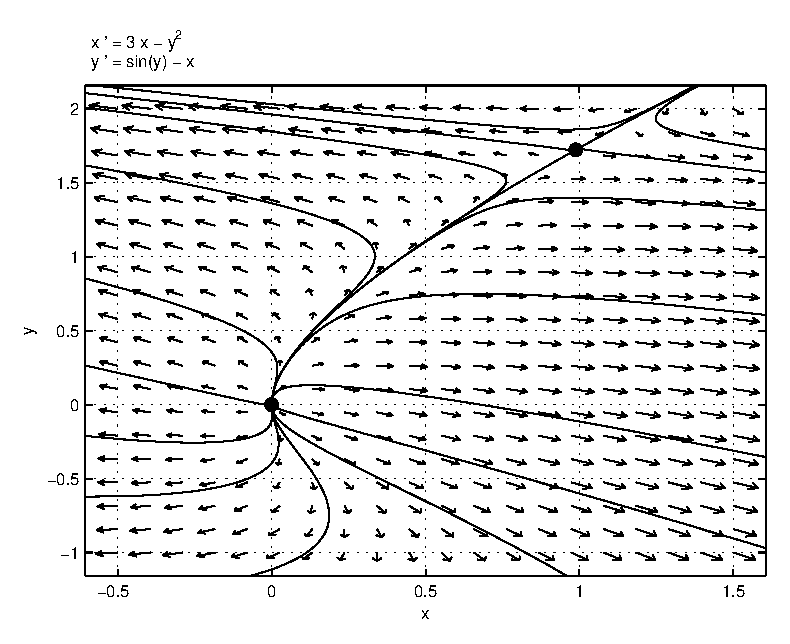
\includegraphics[width=5in]{pplane_plots/NonlinExample1.ps}
}
\caption{Phase portrait for system \eqref{eqn:nonlinexample1}.}
\label{fig:nonlinexample1}
\end{figure}
  The Jacobian matrix is
\begin{equation}
  J = \begin{bmatrix}
           3 &  -2y \\
	   -1 & \cos(y)
      \end{bmatrix}
\end{equation}
and at $(0,0)$, this is
\begin{equation}
  J = \begin{bmatrix}
           3 &  0 \\
	   -1 & 1
      \end{bmatrix}.
\end{equation}
The eigenvalues are $\lambda_1=1$ and $\lambda_2=3$.
Both $\lambda_1>0$ and $\lambda_2>0$, so the origin
in the linearization is a \emph{source}.
Since the real part of both eigenvalues is nonzero,
we conclude that the equilibrium $(0,0)$ of the original
nonlinear equations is also a source.
\emph{Near $(0,0)$}, the linearization provides a
good approximation to the nonlinear system.
The image on the left in Figure~\ref{fig:nonlinexample1compare}
shows the phase portrait of \eqref{eqn:nonlinexample1}
near $(0,0)$, and the image on the right
is the phase portrait of the linearization at $(0,0)$.
\begin{figure}
\centerline{%
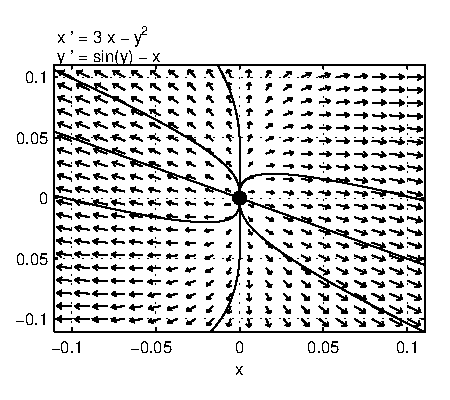
\includegraphics[width=2.5in]{pplane_plots/NonlinExample1detail.ps}
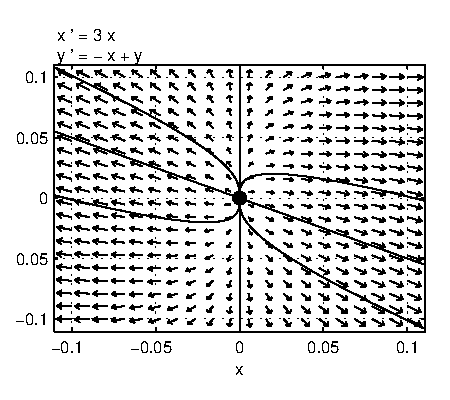
\includegraphics[width=2.5in]{pplane_plots/NonlinExample1lin.ps}
}
\caption{On the left is the phase portrait of
\eqref{eqn:nonlinexample1} near $(0,0)$, and on the
right is the phase portrait of the linearization
at $(0,0)$.  They are almost the same.  If we zoomed
in closer, they would appear even more similar.}
\label{fig:nonlinexample1compare}
\end{figure}
%
%
\paragraph{Example.}
The system of differential equations
\begin{equation}
\begin{split}
  \frac{dx}{dt} & = 2x - y -x^2 \\
  \frac{dy}{dt} & = x - 2y + y^2
\end{split}
\end{equation}
has equilibria at $(0,0)$ and $(1,1)$.
The Jacobian matrix is
\begin{equation}
  J = \begin{bmatrix}
           2-2x & -1 \\
	   1 & -2 + 2y
      \end{bmatrix}
\end{equation}

At $(0,0)$, this is
\begin{equation}
  J = \begin{bmatrix}
           2 & -1 \\
	   1 & -2
      \end{bmatrix}
\end{equation}
This matrix has eigenvalues $\lambda_1 = -\sqrt{3}$ 
and $\lambda_2 = \sqrt{3}$, so the
origin of the  linearized system is a saddle point.
Both eigenvalues are real and nonzero,
so we conclude that the equilibrium
$(0,0)$ of the nonlinear system is also a saddle point.

At $(1,1)$, the Jacobian matrix is
\begin{equation}
  J = \begin{bmatrix}
           0 & -1 \\
	   1 & 0
      \end{bmatrix}
\end{equation}
This matrix has eigenvalues $\lambda=\pm i$,
so the linearization results in a \emph{center}.
Because the real parts of the eigenvalues are
zero, we can \emph{not} conclude that $(1,1)$
is actually a center in the nonlinear system.
Trajectories near $(1,1)$ will rotate around $(1,1)$, but
the linearization can not tell us if these trajectories
actually form closed curves.
The trajectories might, in fact, slowly spiral
towards or away from $(1,1)$.

%
\section{Periodic Solutions}
%
\section{Higher Dimensional Systems}
\[
  \dot{\BX} = \BF(\BX)
\]
\paragraph{Example.}
\emph{Do a 3D example: solve for equilibria, find the
Jacobian, determine stability.  At least one point
should require numerical evaluation of the equilibrium
and of the eigenvalues of the Jacobian.}
\paragraph{Chaos.} Just an example...
%
%
%%%%%%%%%%%%%%%%%%%%%%%%%%%%%%%%%%%%%%%%%%%%%%%%%%%%%%%%%%%
%

\chapter[Dimensional Analysis]{Dimensional Analysis and Nondimensionalization}
\section{Dimensions and Units}
\section{Nondimensional Equations and Parameters}
\section{Exercises}
%
%
%%%%%%%%%%%%%%%%%%%%%%%%%%%%%%%%%%%%%%%%%%%%%%%%%%%%%%%%%%%
%

\chapter{Applications of Differential Equations}
%
In this chapter, we developed models using differential
equations for a wide variety of systems.
We include problems from a wide variety of fields:
\begin{itemize}
\item \emph{Economics}: Solow growth model
\item \emph{Population Dynamics}: predator-prey, competing species
\item \emph{War and Peace}: Lanchester battle model, Richardson's arms
race model
\item \emph{Love Affairs}: a variation of Romeo and Juliet, Rinaldi's
model of Petrarch's love for Laura
\item \emph{Epidemiology}: the SI, SIR, and SIQR models
\end{itemize}
%
\section{Solow's Economic Growth Model\index{Solow growth model}}
We consider a model from macroeconomics.
Let $K$ be the capital,%
\footnote{\emph{Capital} includes things that are owned to be used
in production, such as buildings and manufacturing equipment.}%
~$L$ the labor, and $Q$ the production output of an economy.
We are interested in a \emph{dynamic} problem, so $K(t)$, $L(t)$ and
$Q(t)$ are all functions of time, but we will suppress the $t$ argument.
In elementary economics, one learns that a common assumption is that
$Q$ can be expressed as function of $K$ and $L$:
\begin{equation}
   Q = f(K,L).
   \label{EQN:PROD}
\end{equation}
%We make the reasonable assumptions that $f_K > 0$ and $f_L > 0$.
%(The subscript denotes a partial derivative: $f_K = \partial f/\partial K$.)
%These assumptions mean that $Q$ increases if either $K$ or $L$ increases.
%That is, with more capital or more labor, we can produce more.
%We also assume that $f_{KK} < 0$ and $f_{LL} < 0$.
%These assumptions say that $f$ has \emph{diminishing returns} to the
%inputs $K$ and $L$.  In other words, the larger $K$ is, the less is the
%effect of increasing $K$, and the same holds for $L$.
We assume that $f$ has, using economics terminology,
\emph{constant returns to scale}.  Mathematically, this means
that multiplying $K$ and $L$ by the same amount results in $Q$ being
multiplied by the same amount.  That is, for any constant $b$,
\[
   f(bK,bL) = bf(K,L).
\]
For example, the Cobb-Douglas function\index{Cobb-Douglas function}
$f(K,L) = K^{1/3}L^{2/3}$
satisfies this assumption. 

We make two more assumptions.
We assume that a constant proportion of $Q$ is invested in capital.
This means that the \emph{rate of change} of $K$ is proportional to
$Q$:
\begin{equation}
    \frac{dK}{dt} = s Q,
\label{EQN:DKDT}
\end{equation}
where $s > 0$ is the proportionality constant.
We also assume that the labor force is growing according
to the equation
\begin{equation}
   \frac{dL}{dt} = \lambda L,
   \label{EQN:DLDT}
\end{equation}
where $\lambda > 0$ is the growth rate.  (As you know, this is a simple
first order equation for $L$ which we can solve to find 
$L = L_0 e^{\lambda t}$.)

Now we will combine equations \eqref{EQN:PROD}, \eqref{EQN:DKDT},
and \eqref{EQN:DLDT} to obtain a first order differential equation.
First we express the relation $Q=f(K,L)$ in a different form.
Because $f$ has constant returns to scale, we can write
\begin{equation}
   Q = f(K,L) = f\left(L\frac{K}{L},L\right) 
        = Lf\left(\frac{K}{L},1\right) = Lg(k),
   \label{EQN:QG}
\end{equation}
or
\begin{equation}
  \frac{Q}{L} = g(k)
\end{equation}
where we have introduced a new variable $k = K/L$
(so $k$ is the \emph{ratio} of capital to labor),
and we have defined a new function $g(k) = f(k,1)$.
By differentiating the relation $K = kL$ we obtain
\begin{equation}
   \frac{dK}{dt}  = k\frac{dL}{dt} + \frac{dk}{dt} L
\end{equation}
so
\begin{equation}
\begin{split}
   \frac{dk}{dt} & = \frac{1}{L} \left(\frac{dK}{dt} - \frac{dL}{dt} k\right) \\
                    & = \frac{1}{L} \left( sQ - \lambda L k \right) \\
                    & = s \frac{Q}{L} - \lambda k \\
                    & = s g(k) - \lambda k .
\end{split}
\end{equation}
Thus we have the \emph{Solow Growth Model} \cite{Solow}\index{Solow growth model}
\begin{equation}
  \frac{dk}{dt} = s g(k) - \lambda k
\end{equation}
which models the growth of the ratio of capital to labor
under the assumptions given earlier.

As an example, let's take the production function to be a
Cobb-Douglas function $f(K,L) = K^{1/3}L^{2/3}$.
Then $g(k) = f(k,1) = k^{1/3}$, and the differential equation for
$k$ is
\begin{equation}
   \frac{dk}{dt} = sk^{1/3} - \lambda k .
\label{eqn:solowcobb}
\end{equation}
By solving
\[
   sk^{1/3} - \lambda k = 0,
\]
we find the equilibrium solutions to be $k=0$ or $k=(s/\lambda)^{3/2}$.

The following plot shows the graph of $\frac{dk}{dt}$ versus $k$ when $s=1$ and
 $\lambda=1$.

%\centerline{\includegraphics[width=2.75in,angle=270]{hw01n4b.eps}}
\centerline{\fbox{PLOT HERE!}}

%\vspace{0.25in}
\noindent
Changing $\lambda$ or $s$ will change the scale
(and the numerical value of the non-zero equilibrium),
but the graph of $dk/dt$ versus $k$ will always have the
same qualitative shape as the graph shown above.

We can see that if $k>0$ is small, $k$
will increase, so the equilibrium $k=0$ is \emph{unstable}.
The graph of $k(t)$ will have an inflection point when $k$ reaches
$\left(\frac{s}{3\lambda}\right)^{3/2}$ (where $dk/dt$ has its maximum).
$k$ will then converge asymptotically to the non-zero equilibrium.

The equilibrium $k=(s/\lambda)^{3/2}$ is \emph{asymptotically stable}:
any solution that starts near the equilibrium will converge to the equilibrium
as $t\rightarrow \infty$.
In fact, \emph{all} solutions with $k(0)>0$ will converge asymptotically to this
equilibrium.

A \emph{direction field}\index{direction field} of a first order differential equation is created by
taking a grid of $(t,k)$ values, evaluating the right side of the differential
equation at each point in the grid to find the slope of the solution $k(t)$
through that point, and then plotting a short line segment with that slope
at the point.
The following shows a direction field and some solutions
of \eqref{eqn:solowcobb} when $s=1$ and $\lambda=1$.

%\centerline{\includegraphics[width=4in,angle=270]{hw01n4dirfield.eps}}
\centerline{\fbox{DIRECTION FIELD HERE!}}

\vspace{0.25in}

What does this mean in terms of the capital $K$ and the labor $L$?
Since $k(t) = K(t)/L(t)$, and $L(t) = L_0e^{\lambda t}$, if $k(t)$ converges to an
asymptotically stable equilibrium $k_1$, then $K(t)$ must behave asymptotically like
$k_1  L(t)$.  This means that, in the long term, $K(t)$ must 
grow exponentially, with the
same exponent as $L(t)$.
This model predicts that in the long term, capital will grow
exponentially along with the labor.
If, for example, the capital is too low, it will rapidly increase until it becomes
approximately proportional to the labor, and then it will settle into a long term behavior in
which capital remains proportional to the labor.

%
\section{Predator-Prey\index{predator-prey}}
%
\section{Competing Species\index{competing species}}
%
We consider an example that models the populations
of two species that are competing for a common resource.
In the absence of the other species, each species
grows according to a logistic equation.
However, the presence of one species lowers
the \emph{per capita} growth rate of the other species.
One way to write the equations for this system
is
\begin{equation}
\begin{split}
  \frac{dx}{dt} & = r_1\left(1-\frac{x}{K_1}-\beta_1 y\right)x \\
  \frac{dy}{dt} & = r_2\left(1-\frac{y}{K_2}-\beta_2 x\right)y
\end{split}
\end{equation}
Note that if $y(0)=0$, then $y(t)$ remains $0$, and
the equation for $x(t)$ is
\begin{equation}
    \frac{dx}{dt} = r_1 \left(1-\frac{x}{K_1}\right),
\end{equation}
which is the familiar logistic equation.
Similarly, if $x(0)=0$, then $x(t)$ remains $0$ and
$y(t)$ is governed by a logistic equation.

Let's do a careful analysis of a specific example,
in which $r_1 = 1$, $K_1 = 1$, $\beta_1 = 1$, 
$r_2 = 3/4$, $K_2 = 3/4$, and $\beta_2 = 2/3$.
The differential equations are
\begin{equation}
\begin{split}
  \frac{dx}{dt} & = (1-x-y)x \\
  \frac{dy}{dt} & = \frac{3}{4}\left(1 -\frac{4}{3}y - \frac{2}{3}x\right)y .
\end{split}
\label{eqn:compspecexample}
\end{equation}
We'll find the equilibria, find the linearization at each
equilibrium to determine the behavior near each one, and then
use the nullclines of~\eqref{eqn:compspecexample} to understand
what happens in the phase plane ``far away'' from the equilibria.

\paragraph{Equilibria.}
To find the equilibria, we must solve
\begin{equation}
\begin{split}
(1-x-y)x & = 0 \\
\frac{3}{4}\left(1 -\frac{4}{3}y - \frac{2}{3}x\right)y & = 0.
\end{split}
\label{eqn:exampleequil}
\end{equation}
The first equation holds if $x=0$ or $y = 1-x$.
We consider each case separately in the second equation.
\begin{itemize}
\item
If $x=0$, then the second equation of~\eqref{eqn:exampleequil} implies
$y=0$ or $y=\frac{3}{4}$.

So two equilibria are $(0,0)$ and $(0,3/4)$.
\item
If $y=1-x$, then the second equation
of~\eqref{eqn:exampleequil} implies
\begin{equation}
  \left(1-\frac{4}{3}(1-x) - \frac{2}{3}x\right)(1-x) = 0
  \implies x=1 \quad \textrm{or} \quad x=\frac{1}{2}.
\end{equation}
So two equilibria are $(1,0)$ and $(1/2,1/2)$.
\end{itemize}

\paragraph{Linearization at each equilibrium.}
We have found the following equilibria: $(0,0)$, $(0,3/4)$, $(1,0)$, $(1/2,1/2)$.
We now determine the behavior of~\eqref{eqn:compspecexample}
near each equilibrium by finding the linearization at each
equilibrium.
We will need the Jacobian matrix:
\begin{equation}
  J = \begin{bmatrix}
          1-2x-y & -x \\
	  -\frac{1}{2}y & \frac{3}{4}-2y-\frac{1}{2}x
      \end{bmatrix}
\end{equation}
For each equilibrium, we will find the Jacobian matrix
and plot the phase portrait of the linearization.
We make two remarks about the phase portraits of the linearized
systems:
\begin{enumerate}
\item
Recall from the notes on ``Linearization'' that we
used the local coordinates $(u,v)$ for the linearization.
In a linear system, the scale of the coordinates is not
important: if you zoom in on the origin of a linear system,
the phase portrait will look exactly the same.
So, in the following phase portraits of the linearizations,
the ranges on the axis are  from $-1$ to $1$.  These
are \emph{not} the actual $x$ and $y$ ranges.
\item
In a population model such as this, $x<0$ and $y<0$
are not relevant.  However, we will still plot negative
values in the linearization.  It seems easier to simply
plot the linear phase portrait, ignoring the actual
meaning until later.  Also, recall that the linearized
system is expressed in coordinates measured relative
to the equilibrium.  If a coordinate of the equilibrium
is positive, then a negative value of the corresponding
local coordinates means that the population is less than
the equilibrium value. It does not necessarily mean that
the actual population is negative.
\end{enumerate}

\medskip

At $(0,0)$, the Jacobian matrix is
\begin{equation}
  J = \begin{bmatrix}
          1 & 0 \\
	  0 & \frac{3}{4} \\
      \end{bmatrix} .
\end{equation}
The eigenvalues are $\lambda_1 = 3/4$ and $\lambda_2 = 1$, with
corresponding eigenvectors
\[
  \BV_1 = \begin{bmatrix} 0 \\ 1 \end{bmatrix}
  \quad \textrm{and}\quad 
  \BV_2 = \begin{bmatrix} 1 \\ 0 \end{bmatrix}.
\]
Since $\lambda_1 > 0$ and $\lambda_2 > 0$,
the equilibrium $(0,0)$ is a
\emph{source}.  The trajectories come out of $(0,0)$
tangent to the eigenvector $\BV_1$.
The phase portrait of the linearization at $(0,0)$ is
shown in Figure~\ref{fig:CompSpecLinPlots}(a).
%\centerline{%
%\includegraphics{matlab/LinCS1.eps}
%}
%\noindent
If we were to ``zoom in'' on the point $(0,0)$
in~\eqref{eqn:compspecexample}, this is what the 
phase portrait would look like.

%\medskip

At $(1,0)$, the Jacobian matrix is
\begin{equation}
  J = \begin{bmatrix}
          -1 & -1 \\
	  0 & \frac{1}{2} \\
      \end{bmatrix}.
\end{equation}
The eigenvalues are $\lambda_1 = -1$ and $\lambda_2 = 1/2$,
with corresponding eigenvectors
\[
  \BV_1 = \begin{bmatrix} 1 \\ 0 \end{bmatrix}
  \quad \textrm{and} \quad
  \BV_2 = \begin{bmatrix} 1 \\ -3/2 \end{bmatrix}.
\]
Since $\lambda_1 < 0$ and $\lambda_2 > 0$, the equilibrium
$(1,0)$ is a \emph{saddle point}.
The phase portrait of the linearization at $(1,0)$ is
shown in Figure~\ref{fig:CompSpecLinPlots}(b).

%\centerline{%
%\includegraphics{matlab/LinCS2.eps}
%}

%\medskip

At $(0,3/4)$, the Jacobian matrix is
\begin{equation}
  J = \begin{bmatrix}
          \frac{1}{4} & 0 \\
	  -\frac{3}{8} & -\frac{3}{4} \\
      \end{bmatrix}.
\end{equation}
The eigenvalues are $\lambda_1 = -\frac{3}{4}$ and
$\lambda_2 = \frac{1}{4}$,
with corresponding eigenvectors
\[
  \BV_1 = \begin{bmatrix} 1 \\ -3/8 \end{bmatrix}
  \quad \textrm{and}\quad 
  \BV_2 = \begin{bmatrix} 0 \\ 1 \end{bmatrix}.
\]
Since $\lambda_1 < 0$ and $\lambda_2 > 0$,
the equilibrium $(0,3/4)$
is a \emph{saddle point}.
The phase portrait of the linearization at $(0,3/4)$ is
shown in Figure~\ref{fig:CompSpecLinPlots}(c).

%\centerline{%
%\includegraphics{matlab/LinCS3.eps}
%}

%\medskip

At $(1/2,1/2)$, the Jacobian matrix is
\begin{equation}
  J = \begin{bmatrix}
          -\frac{1}{2} & -\frac{1}{2} \\
	  -\frac{1}{4} & -\frac{1}{2} \\
      \end{bmatrix}.
\end{equation}
The eigenvalues are
$\lambda_1 = \frac{-2-\sqrt{2}}{4} \approx -0.853 < 0$
and $\lambda_2 = \frac{-2+\sqrt{2}}{4} \approx -0.147 < 0$,
with corresponding eigenvectors
\[
  \BV_1 = \begin{bmatrix} \sqrt{2} \\ 1 \end{bmatrix}
  \quad \textrm{and}\quad
  \BV_2 = \begin{bmatrix} \sqrt{2} \\ -1 \end{bmatrix}.
\]
Since both eigenvalues are negative,
the equilibrium at $(1/2,1/2)$ is a \emph{sink}.
The phase portrait of the linearization at $(1/2,1/2)$ is
shown in Figure~\ref{fig:CompSpecLinPlots}(d)

%\centerline{%
%\includegraphics{matlab/LinCS4.eps}
%}

%\medskip

\begin{figure}
\centerline{\includegraphics[width=2.5in]{matlab/LinCS1.eps}\includegraphics[width=2.5in]{matlab/LinCS2.eps}}
\vspace{-0.2in}
\centerline{\hspace{0.2in}\textbf{(a)}\hspace{2.1in}\textbf{(b)}}
\centerline{\includegraphics[width=2.5in]{matlab/LinCS3.eps}\includegraphics[width=2.5in]{matlab/LinCS4.eps}}
\vspace{-0.2in}
\centerline{\hspace{0.2in}\textbf{(c)}\hspace{2.1in}\textbf{(d)}}
\caption{Phase portraits of the linearizations at each equilibrium point
of the competing species example:
(a) at $(0,0)$; (b) at $(1,0)$; (c) at $(0,3/4)$; (d) at $(1/2,1/2)$.}
\label{fig:CompSpecLinPlots}
\end{figure}



\paragraph{Nullclines.}
Since the eigenvalues at each linearization
all had nonzero real parts, each linearization
provides a good approximation to the behavior
of~\eqref{eqn:compspecexample} near the corresponding
equilibrium point.
However, the local linearizations do not tell us what is
happening in the phase plane far from the equilibria.
In a planar system such as this, the nullclines
can provide useful information about the phase portrait.

The $x$ nullcline is given by
\begin{equation}
   (1-x-y)x = 0 \implies x=0 \quad\textrm{or}\quad y = 1-x.
\end{equation}
So $\frac{dx}{dt}=0$ on the lines $x=0$
and $y=1-x$.\footnote{In this example, and in all
the planar linear systems that we have studied,
the nullclines are straight lines. This is not true in general;
nullclines can be curves.}

The $y$ nullcline is given by
\begin{equation}
  \frac{3}{4}\left(1-\frac{4}{3}y - \frac{2}{3} x\right)y = 0
\end{equation}
which gives the lines
\begin{equation}
  y = 0 \quad \textrm{or} \quad y = \frac{3}{4} - \frac{1}{2}x.
\end{equation}
On these lines, $\frac{dy}{dt}=0$.

The nullclines give the points in the plane where 
$\frac{dx}{dt}=0$ or $\frac{dy}{dt}=0$.
They form the boundaries of regions in the plane
where $\frac{dx}{dt}$ and $\frac{dy}{dt}$ do not change sign.
This can be very useful information.
For example, if we know that in a certain region,
$\frac{dx}{dt} > 0$ and $\frac{dy}{dt}>0$, we know that all
vectors of the vector field point ``up and to the right'';
this means all trajectories move up and to the right.
If this region is in the first quadrant, it implies that
all trajectories move away from the origin.

In the following plot, the nullclines (that are not coordinate
axes) are plotted with dashed lines, and trajectories
are plotted as solid lines.  Since our equations give 
a model for two species, we only include the first quadrant.
Negatives values would not be meaningful, so we do not include them.

\smallskip
\centerline{%
\fbox{\includegraphics[width=4.5in]{matlab/CompSpec.eps}}
}

\medskip
\noindent
In the region labeled \textsf{\textbf{A}},
$\frac{dx}{dt}<0$ and $\frac{dy}{dt}<0$.
All trajectories in this region (which extends out to infinity)
must move down and to the left.  This implies that
all these trajectories must either cross the $x$ or $y$ axes,
or cross the nullclines that form the boundaries between
\textsf{\textbf{A}} and \textsf{\textbf{B}}
and between \textsf{\textbf{A}} and \textsf{\textbf{D}}.
But the coordinate axes are themselves solutions,
so solutions that do not start on the coordinate axes
can not cross the axes.  Thus any trajectory that begins in
\textsf{\textbf{A}} must eventually cross into
\textsf{\textbf{B}} or \textsf{\textbf{D}}
(or, in one special case, converge to the equilibrium
at $(1/2,1/2)$).

Now consider trajectories in \textsf{\textbf{B}}.
In \textsf{\textbf{B}}, we have
$\frac{dx}{dt} > 0$ and $\frac{dy}{dt} < 0$.
All trajectories in this region move down and to the right.
They can not cross either of the nullclines that
form the upper and lower boundaries of the region,
because the vector field on these nullclines points
\emph{into} \textsf{\textbf{B}}.  Therefore,
\emph{all trajectories in \textsf{\textbf{B}} must
converge to $(1/2,1/2)$}.

A similar argument applies to \textsf{\textbf{D}},
where $\frac{dx}{dt} < 0$ and $\frac{dy}{dt} >0$.
In this region, all trajectories move up and to the left,
but they can't cross the nullclines, so
\emph{all trajectories in \textsf{\textbf{D}} must
converge to $(1/2,1/2)$}.

Finally, in \textsf{\textbf{C}} we have
$\frac{dx}{dt} >0$ and $\frac{dy}{dt} > 0$.
All trajectories in this region move up and to the right.
Therefore, they must all eventually cross into
\textsf{\textbf{B}} or \textsf{\textbf{D}}, except
for the special trajectory in \textsf{\textbf{C}}
that converges to $(1/2,1/2)$.

Our conclusion is that any trajectory that begins in the
first quadrant, with $x(0)>0$ and $y(0)>0$, must
converge to $(1/2,1/2)$. Note that we have concluded this
without actually solving the differential equations
given in~\eqref{eqn:compspecexample}.
Thus, this population model
predicts that the two species will co-exist in 
a stable equilibrium.
(But different parameters values can lead to different
conclusions.)
%
%
\section{Battle of Attrition--The Lanchester Model}
\index{Lanchester model}
%
We consider a model of a battle in which the opponents
simply blast away at each other until one side is wiped
out.
This model was proposed by Lanchester (ref...).
This is \emph{not} a realistic model of modern warfare!
(It has been suggested as a model for the battles that
occur between colonies of ants...\emph{find this reference!})
In this model $x(t)$ and $y(t)$ are the sizes of the
opposing armies at time $t$.
As the battle rages, the losses incurred by army $x$
are simply proportional to the size of army $y$,
and the losses incurred by army $y$ are proportional
to the size of army $x$ (but not necessarily with
the same proportionality constant).
That is,
\begin{equation}
\begin{split}
   \frac{dx}{dt} & = - \alpha y \\
   \frac{dy}{dt} & = - \beta x
\end{split}
\end{equation}
where $\alpha$ and $\beta$ are positive constants.
This is a planar linear system.
The coefficient matrix is
\begin{equation}
  A = \begin{bmatrix} 0 & -\alpha \\ -\beta & 0 \end{bmatrix}.
\end{equation}
The eigenvalues are $\lambda_1 = -\sqrt{\alpha\beta}$
and $\lambda_2 = \sqrt{\alpha\beta}$,
so we know that the origin $(0,0)$ is a saddle point.
A corresponding set of eigevectors are
\[
  \BV_1 = \begin{bmatrix} 1 \\ -\sqrt{\frac{\beta}{\alpha}}\end{bmatrix}
  \quad \textrm{and}\quad
  \BV_2 = \begin{bmatrix} 1 \\ \sqrt{\frac{\beta}{\alpha}}\end{bmatrix}.
\]
The $x$ nullcline is $y=0$, which means that trajectories
cross the $x$ axis vertically. Similarly, the $y$ nullcline is
$x=0$, so trajectories cross the $y$ axis horizontally.
Since the nullclines are the axes, we know that in the first
quadrant, $dx/dt < 0$ and $dy/dt < 0$, so for any initial
condition in the first quadrant, the trajectory will eventually
cross either the $x$ or $y$ axis. If the initial condition
happens to be in the eigenspace associated with the negative
eigenvalue $\lambda_1$, the trajectory will converge to
$(0,0)$. (In this exceptional case, the armies wipe each
other out!)
This eigenspace is given by the line
\begin{equation}
  y = \sqrt{\frac{\beta}{\alpha}}\, x.
\end{equation}
If the initial condition is above the $\lambda_1$ eigenspace
(so $y_0 > \sqrt{\frac{\beta}{\alpha}}\, x_0$), then
$y$ wins, and if the initial condition is below this line,
then $x$ wins.

There is a different approach we can take for studying
this system.
By multiplying the first equation by $2\beta x$ and the
second by $-2\alpha y$, we obtain
\begin{equation}
\begin{split}
 2\beta x\frac{dx}{dt} & = -2 \alpha \beta x y \\
 -2\alpha y\frac{dy}{dt} & = 2 \alpha \beta x y.
\end{split}
\end{equation}
Then adding these equations results in
\begin{equation}
   2\beta x\frac{dx}{dt} -2\alpha y\frac{dy}{dt} = 0.
\end{equation}
We note that the left side of this equation is
the $t$ derivative of $\beta x^2 - \alpha y^2$.
So we'll integrate from $0$ to $t$:
\begin{equation}
   \int_0^t \left(2\beta x\frac{dx}{dt} -2\alpha y\frac{dy}{dt}\right)\, ds = \int_0^t 0 \, ds = 0.
\end{equation}
which gives
\begin{equation}
\begin{split}
  \left.\beta x^2(s) - \alpha y^2(s)\right|_{s=0}^{s=t} & = 0 \\
   \beta x^2(t) - \alpha y^2(t) - (\beta x^2(0) - \alpha y^2(0)) & = 0 \\
      \beta x^2(t) - \alpha y^2(t) & = \beta x^2(0) - \alpha y^2(0) =
         \beta x_0^2 - \alpha y_0^2 \\
\end{split}
\end{equation}
By dropping the explicit $t$ dependence of $x(t)$
and $y(t)$, we obtain
\begin{equation}
   \beta x^2 - \alpha y^2 = \beta x_0^2 - \alpha y_0^2.
   \label{eqn:lanchester_hyperbola}
\end{equation}
This is the equation of a hyperbola in the $(x,y)$ plane.
Whether the hyperbola crosses the $x$ or $y$ axis is
determined by the sign of
$\beta x_0^2 - \alpha y_0^2$.
If this value is positive, then the hyperbola
crosses the positive $x$ axis
at $x=\sqrt{x_0^2 - \frac{\alpha}{\beta} y_0^2}$.
If $\beta x_0^2 - \alpha y_0^2$
is negative, then the hyperbola
crosses the $y$ axis at
$y = \sqrt{y_0^2 - \frac{\alpha}{\beta} x_0^2}$.
Thus, if we know the initial sizes of the armies
and the constants $\alpha$ and $\beta$, we can
easily determine which army will win, and what the
size of the winning army will be at the end of the
battle.
\section{Arms Race}
%
\section{Romeo and Juliet\index{Romeo}\index{Juliet}}
\section{Laura and Petrarch\index{Laura}\index{Petrarch}}
%
\section{Epidemiology and the SI Model\index{SI model}}

In this chapter we consider some models of the spread of disease.
These models lead to systems of differential equations.

We will assume that the population has a fixed size $N$.
We also assume that the people (or animals) in the population
intermingle sufficiently fast that we do not have to take
into account the geography of the community.
Our model will not attempt to deal with the geographic spread
of the disease. It will only look at the total number of
people infected within the given population.

\paragraph{The SI Model.}
In the simplest model, we will consider just two classes
of people: those who have been infected, and those who have
not.
Let $I(t)$ be the number of people infected at time $t$.
(We'll often call this group the ``infectives''.)
Let $S(t)$ be the number of people who have not
been infected, but are susceptible to the disease.
In our simplest model, we will assume that no one is immune,
so each person is susceptible, or infected.  Thus
\[
   S+I = N.
\]
So we suppose we have a population of interacting people,
some of whom are infected.  How fast will the susceptible
people become infected?  We can think of this in terms
of probability.  If we pick two people at random from
the population, what is the probability that one is
susceptible and the other is infected? The probability
of picking a susceptible person is $S/N$, and the probability
of picking an infective is $I/N$.  For large $N$ (i.e. for
$N-1\approx N$), the probability that two random
people will consist of one susceptible and one infected
is $2(S/N)(I/N) = rSI$, where $r$ is a constant.
Of course, an infective coming into contact
with a susceptible does not necessarily spread the disease
to the susceptible.
We can take the ``infectiousness'' of the disease into
account by adjusting the constant $r$.
The gist of this argument is that we expect the rate
of change of $S$ (which is the same as the rate of
the spread of the disease in this model) to be proportional
to the \emph{product} $SI$.
We assume $r>0$.  Then the equation that gives the
rate of change of $S$ is
\begin{equation}
  \frac{dS}{dt} = -r S I.
\label{eqn:SI_S}
\end{equation}
The minus sign accounts for this being a \emph{decrease}
in the number of susceptibles.
In this simplest model, the spread of the disease
means people move from being susceptible to
infected, so any loss in $S$ must have a corresponding
gain in $I$.  Thus
\begin{equation}
  \frac{dI}{dt} = r S I.
\label{eqn:SI_I}
\end{equation}
Equations \eqref{eqn:SI_S} and \eqref{eqn:SI_I}
constitute a \emph{system of differential equations}.
Many dynamical processes are modeled with systems of differential
equations; we'll see many more in this course.
In fact, this is a \emph{nonlinear} system.
Typically, nonlinear systems
that arise in the real world can not be solved analytically.
It turns out that this particular system can be solved.

First, we check that the total population remains constant by adding these
two equations.  We find
\begin{equation}
  \frac{dS}{dt} + \frac{dI}{dt} = 0
\end{equation}
and integrating from $0$ to $t$ gives
\begin{equation}
  S(t) + I(t) = S(0)+I(0).
\end{equation}
The initial population was $N$, so we have
$S(t)+I(t)=N$.
This means we can replace $S$ in \eqref{eqn:SI_I} with
$N-I$ to obtain
\begin{equation}
  \frac{dI}{dt} = r(N-I)I.
\end{equation}
This is just another version of the logistic equation, 
which we know how to solve.
If $I(0)>0$, we know that $I(t)$ will approach the
equilibrium $N$ as $t\rightarrow\infty$.
Thus, this simple model predicts that
everyone will become infected, no matter how small
the initial population of infectives.

\section{The SIS Model\index{SIS model}}
%
% Perhaps the SIS model could be given as an exercise:
% state the assumption, and then have the student give
% the equations.
%
For some diseases, surviving an infection
does not guarantee immunity from subsequent infections.
Infectives can recover,
but once they have recovered, they return to the
susceptible pool... 


\section{The SIR Model\index{SIR model}}
For many diseases, people recover after being infected,
and from then on they are immune to the disease.
To incorporate this into our model of the spread of
a disease, we consider a third class of \emph{recovered}
people. (Calling them the recovered people is the
optimistic point of view.  It turns out that the
model is the same if we interpret this group as
\emph{removed}, meaning deceased.)

We assume that the rate at which the infected
group changes to recovered is proportional to
the number of infected people.

\emph{Why? ...}

So, if we have a group of infectives, and no
one else is becoming infected, the equation
for $I(t)$ is
\begin{equation}
  \frac{dI}{dt} = -\gamma I,
\end{equation}
where $\gamma > 0$ is the constant of proportionality.
The parameter $\gamma$ depends on how fast people
typically recover from the disease.
The decrease in $I$ because of recovery results
in a corresponding increase in $R(t)$.
Putting this all together, we obtain the
$SIR$ model:\index{SIR model}
\begin{equation}
\begin{split}
   \frac{dS}{dt} & = -r S I \\
   \frac{dI}{dt} & = r S I - \gamma I \\
   \frac{dR}{dt} & = \gamma I
\end{split}
\label{eqn:SIR}
\end{equation}
As in the $SI$ model, we have assumed that the total
population remains constant.  This is apparent in the equations:
add them all together to find
\begin{equation}
   \frac{dS}{dt} + \frac{dI}{dt} + \frac{dR}{dt} = 0
   \quad \textrm{which implies} \quad
   S(t) + I(t) + R(t) = N.
\end{equation}
Also note that $R$ does not appear in the first two equations
of \eqref{eqn:SIR}.  This means we can analyze the equations
for $S$ and $I$, and then infer the behavior of $R$ afterwards.

\medskip
\noindent
\emph{To be continued...}


\section{The SIQR Model\index{SIQR model}}
%
%
%%%%%%%%%%%%%%%%%%%%%%%%%%%%%%%%%%%%%%%%%%%%%%%%%%%%%%%%%%%
%

\chapter{Discrete Maps}
%
\section{Modeling with Discrete Maps}
%
\section{One-Dimensional Maps}
\label{sec:OneDimMaps}
We begin with the simplest model of population growth.
Suppose, for example, a population increases by 15 percent each
year.
Let $p_n$ be the population at the end of year $n$, and assume that
$p_0$ is given.
Then an increase of 15 percent each year gives
\begin{equation}
  p_{n+1} = 1.15p_n.
  \label{eqn:pop}
\end{equation}
If $p_0=100$, then $p_1 = 1.15(100) = 115$,
$p_2 = 1.15(115) = 132.3$, $p_3 = 1.15(132.3) = 152.1$, and so on. 
Table~\ref{tbl:popdata} shows the first nine iterations of
this process.
\begin{table}[h]
\centerline{%
\begin{tabular}{|c|l|c|l|}
\hline
 $n$  &  $p_n$ & $n$ & $p_n$ \\ 
\hline
  0  & 100.0  & 5 & 201.1 \\ 
\hline
  1 &  115.0  & 6 & 231.3 \\ 
\hline
  2 &  132.3  & 7 & 266.0 \\ 
\hline
  3 &  152.1  & 8 & 305.9\\ 
\hline
  4 &  174.9  & 9 & 351.8 \\ 
\hline
\end{tabular}
}
\caption{Iteration of the map~\eqref{eqn:pop}, with
$p_0=100$.}
\label{tbl:popdata}
\end{table}
The data is plotted in Figure~\ref{fig:popdataplot}.
\begin{figure}
\centerline{%
\includegraphics{matlab_map1d/popdataplot.eps}
}
\caption{Plot of the data for the simple population growth
model~\eqref{eqn:pop}.  The data is in Table~\ref{tbl:popdata}.}
\label{fig:popdataplot}
\end{figure}

We derive a formula for $p_n$ by noting that
\begin{equation}
\begin{split}
   p_1 & = 1.15p_0 \\
   p_2 & = 1.15p_1 = (1.15)^2 p_0 \\
   p_3 & = 1.15p_2 = (1.15)^3 p_0 \\
       & \vdots \\
   p_n & = (1.15)^n p_0
\end{split}
\end{equation}
Thus we have the familiar ``exponential growth'' of the
population.

More generally, the same argument shows that the solution
to
\begin{equation}
   p_{n+1} = a p_n,
\end{equation}
given $p_0$, is
\begin{equation}
   p_n = a^k p_0.
\label{eqn:psol}
\end{equation}

Let's compare the discrete time map to the continuous time model.
Recall that a first order differential equation
that leads to exponential growth
(or decay) is
\begin{equation}
 \frac{dp}{dt} = r p, \quad\quad p(0) = p_0,
\label{eqn:contpop}
\end{equation}
which has the solution
\begin{equation}
  p(t) = p_0e^{rt} = \left( e^r\right)^t p_0.
\end{equation}
I've written the solution as
$\left(e^r\right)^t p_0$ to make clear the analogy
between the continuous solution and the solution to the discrete
model in \eqref{eqn:psol}.
The term $e^r$ is analogous to $a$, and $t$ is analogous to $n$.

Let's rewrite \eqref{eqn:pop} as
\begin{equation}
  p_{n+1} = (1 + 0.15)p_n = p_n + 0.15p_n
\end{equation}
or
\begin{equation}
  p_{n+1} - p_{n} = 0.15p_n .
\end{equation}
This form of the equation expresses the
\emph{discrete change} in
$p_n$ as a function of $p_n$.
(Such an equation is often called a \emph{difference equation}.)
Compare this to equation~\eqref{eqn:contpop}, which gives the
\emph{instantaneous rate of change} of $p$ as a function
of $p$.

\subsection*{One-dimensional Maps}
The general one-dimensional map has the form
\begin{equation}
   x_{n+1} = f(x_n), \quad \textrm{given $x_0$}.
\label{eqn:onedmap}
\end{equation}
We'll develop several tools for studying such maps.


\subsection*{``Cobwebbing'': The Graphical Iteration Procedure}
There is a simple graphical procedure for generating the
iterations of a one-dimensional map.
As an example, we consider the logistic map
\begin{equation}
   x_{n+1} = rx_n(1-x_n)
\label{eqn:logisticmap}
\end{equation}
where $r > 0$ is a constant.
Table~\ref{tbl:data} shows the first few iterates in the
sequence that results when
$r=2.8$ and $x_0=0.1$.
\begin{table}
\centerline{%
\begin{tabular}{|c|l|c|l|}
\hline
 $n$  &  $x_n$ & $n$ & $x_n$ \\ 
\hline
  0  &  0.1    & 5 & 0.6771 \\ 
\hline
  1 &  0.2520  & 6 & 0.6122 \\ 
\hline
  2 &  0.5278  & 7 & 0.6648 \\ 
\hline
  3 &  0.6978  & 8 & 0.6240 \\ 
\hline
  4 &  0.5904  & 9 & 0.6570 \\ 
\hline
\end{tabular}
}
\caption{Iteration of the logistic map~\eqref{eqn:logisticmap}, with
$r=2.8$ and $x_0=0.1$.}
\label{tbl:data}
\end{table}
%
Figure~\ref{fig:logistic_ts} shows the plot of $x_n$ as a function
of $n$.
%
\begin{figure}
\centerline{\includegraphics{matlab_map1d/logisticmap_timeseries.eps}}
\caption{The first several iterates of the logistic map~\eqref{eqn:logisticmap}
with $r=2.8$ and $x_0=0.1$. This is a plot of the data shown
in Table~\ref{tbl:data}.}
\label{fig:logistic_ts}
\end{figure}
%

The graphical technique for finding the iterations of this map
begins by plotting the graph of the $f(x) = rx(1-x)$, as in
Figure~\ref{fig:logisticmap_example} (where $r=2.8$).
Given $x_0$, we draw a line from the $x=x_0$ on the $x$
axis up the the graph of $x_0$ to obtain $x_1$.
To obtain $x_2$, we need to go to $x=x_1$ on the $x$ axis.
This can be done by drawing a line horizontally from
$(x_0,x_1)$ to the line $y=x$.
See the upper left plot of Figure~\ref{fig:cobwebsequence}.
To find $x_2$, we again draw a line vertically
at $x=x_1$ to the graph, and from the graph we draw a 
line horizontally to $y=x$.
See the upper right plot of Figure~\ref{fig:cobwebsequence}.
We continue this process to generate further iterations,
as in the lower left and right plots of
Figure~\ref{fig:cobwebsequence}.
In these plots, I've included vertical lines from the $x$ axis
up to the graph, but we don't really need these lines.
In practice, the procedure is: 
draw a line vertically
to the graph, then 
draw a line horizontally to $y=x$,  and then repeat
the process.
An example is shown in Figure~\ref{fig:cobwebfinal}.

\begin{figure}
\centerline{\includegraphics[width=3in]{matlab_map1d/logisticmap_example.eps}}
\caption{A graph of the logistic map $rx(1-x)$ for $r=2.8$.}
\label{fig:logisticmap_example}
\end{figure}
%
\begin{figure}
\centerline{%
\includegraphics[width=2.65in]{matlab_map1d/logisticmap_cobweb1.eps}
\includegraphics[width=2.65in]{matlab_map1d/logisticmap_cobweb2.eps}
}
\centerline{%
\includegraphics[width=2.65in]{matlab_map1d/logisticmap_cobweb3.eps}
\includegraphics[width=2.65in]{matlab_map1d/logisticmap_cobweb4.eps}
}
\caption{A sequence of plots that illustrate
``cobwebbing''. The initial point is $x_0=0.1$.}
\label{fig:cobwebsequence}
\end{figure}
%
\begin{figure}
\centerline{%
\includegraphics[width=3.5in]{matlab_map1d/logisticmap_cobwebfinal.eps}
}
\caption{When cobwebbing, we usually don't bother dropping
lines down to the horizontal axis. After the first vertical
line is drawn from $(x_0,x_0)$ to the graph, we draw
a line horizontally to the line
$y=x$, and then another line vertically to graph, and repeat.
This cobweb plot shows
the same data listed in Table~\ref{tbl:data} and plotted in
Figure~\ref{fig:logistic_ts}.}
\label{fig:cobwebfinal} 
\end{figure}
%
%\newpage
\subsection*{Linear Maps}

A \emph{linear} one-dimensional map is
\begin{equation}
   x_{n+1} = a x_n
\end{equation}
where $a$ is a constant.
(The population model \eqref{eqn:pop}
is an example.)
The solution is
\begin{equation}
   x_n = a^n x_0.
\end{equation}
Let's look at how the behavior of the solution
depends on $a$.
\begin{enumerate}
\item If $a > 1$, then $a^n > 0$, and $a^n$ increases without
bound as $n$ increases. So $x_n$ grows exponentially.
\item If $a = 1$, then $a^n=1$ for all $n$, so $x_n = x_0$.
\item If $0 < a < 1$, then $a^n > 0$, and $a^n$ approaches
zero as $n$ increases; $x_n$ decays to zero monotonically.
\item If $a=0$, then $x_n=0$ for all $n > 0$.
\item If $-1 < a < 0$, then $a^n$ alternates sign, and
$a^n$ approaches zero as $n$ increases;
$x_n$  decays to zero while alternating sign.
\item If $a = -1$, then $a^n = (-1)^n$, which is $1$ if $n$
is even and $-1$ if $n$ is odd.  Thus $x_n$ alternates
between $x_0$ and $-x_0$.
\item If $a < -1$, then $a^n$ alternates sign,
and $|a^n|$ increases without bound as $n$ increases.
So $x_n$ alternates sign while $|x_n|$ grows exponentially.
\end{enumerate}
Overall, the magnitude of $x_n$ \emph{grows if} $|a| > 1$,
and \emph{decays if} $|a| < 1$.
Figures~\ref{fig:linearcases_pos}
and \ref{fig:linearcases_neg} show sample plots of $x_n$
and cobweb diagrams for the various cases.
\begin{figure}
\centerline{%
\includegraphics{matlab_map1d/linearcases_pos.eps}
}
\caption{Examples of linear maps, $a \ge 0$. In all cases, $x_0=10$.}
\label{fig:linearcases_pos}
\end{figure}
%
\begin{figure}
\centerline{%
\includegraphics{matlab_map1d/linearcases_neg.eps}
}
\caption{Examples of linear maps, $a < 0$. In all cases, $x_0=10$.}
\label{fig:linearcases_neg}
\end{figure}
%
%
\subsection*{Fixed Points, Stability, Linearization}
A \emph{fixed point} of the map \eqref{eqn:onedmap}
is a point $x^*$ where $f(x^*)=x^*$.
If $x_0=x^*$, then $x_n=x^*$ for all $n>0$, so the fixed points
of $f$ are the constant solutions to \eqref{eqn:onedmap}.

In the logistic map shown in Figure~\ref{fig:logisticmap_example},
we see there are two
points where $f(x)=x$.  These are the points
where the graph of $f$ crosses the line $y=x$.
For the example shown in Figure~\ref{fig:logisticmap_example},
the graph is $f(x) = 2.8x(1-x)$, so to find the fixed points,
we must solve
\begin{equation}
  2.8x(1-x) = x \implies -2.8x^2 + 1.8x = 0
  \implies x = 0 \;\textrm{or}\; x = \frac{1.8}{2.8}
\end{equation}
So the two fixed points are $x=0$ and $x=\frac{1.8}{2.8}\approx 0.643$.

\paragraph{Definition.}
The fixed point $x^*$ is a \emph{sink} or \emph{attractor}
if there is a neighborhood $N$ of $x^*$ such that
$x_n\rightarrow x^*$ for all $x_0$ in $N$.
We also say $x^*$ is \emph{asymptotically stable}.

\paragraph{Definition.}
The fixed point $x^*$ is a \emph{source} or \emph{repellor}
if there is a neighborhood $N$ of $x^*$ such that if $x_0$
is in $N$, then $x_n$ eventually leaves $N$.

\paragraph{Definition.}
The fixed point $x^*$ is \emph{unstable} if for every
neighborhood $N$ of $x^*$, there are points arbitrarily close
to $x^*$ whose iterates leave $N$.

\vspace{0.2cm}
Note that a source is unstable, but an unstable fixed point
is not necessarily a source.  See, for example,
Figure~\ref{fig:noconclusion1}.

\paragraph{Behavior near a fixed point: the linearization.}
Let $x^*$ be a fixed point of \eqref{eqn:onedmap}.
If $x$ is close to $x^*$,
we can approximate $f(x)$ with the tangent line at $x^*$:
\begin{equation}
   f(x) \approx f(x^*) + f'(x^*)(x-x^*).
\end{equation}
Let $u_n = x_n-x^*$ (i.e. $x_n = x^* + u_n$).
Then, by replacing $x_n$ with $x^*+u_n$
in \eqref{eqn:onedmap}, we obtain
\begin{equation}
  x^* + u_{n+1} = f(x^*+u_n) \approx f(x^*)+f'(x^*)u_n.
\end{equation}
Since $f(x^*)=x^*$, we can cancel $x^*$ on the left
and $f(x^*)$ on the right.
We are left with the
\emph{linearization of the map at } $x^*$:
\begin{equation}
  u_{n+1} = f'(x^*)u_n
\end{equation}
This is a linear map.
We have already seen how the solution to the linear
map depends on $a=f'(x^*)$; see Figures~\ref{fig:linearcases_pos}
and \ref{fig:linearcases_neg}.
However, the linearization is just an approximation
to the actual map~\eqref{eqn:onedmap}.
The following theorem tells us when the linear approximation
is ``good enough'' to classify the stability of the
fixed point $x^*$ of \eqref{eqn:onedmap}.

\paragraph{Theorem 1.}
(i) If $|f'(x^*)| < 1$, then $x^*$ is a sink.
(ii) If $|f'(x^*)| > 1$, then $x^*$ is a source.


\paragraph{Example.}
Consider again the logistic map \eqref{eqn:logisticmap}
with $r=2.8$.  The graph is shown in
Figure~\ref{fig:logisticmap_example}, and earlier we found the
fixed points to be $x^*_1=0$ and $x^*_2=\frac{1.8}{2.8}$.
We find
\begin{equation}
  f'(x) = 2.8(1-2x).
\end{equation}
We use Theorem 1 to determine the stability of the fixed points.
\begin{itemize}
\item
At $x^*_1$, we have $f'(0) = 2.8 > 1$, so by Theorem 1,
$x^*_1$ is a source.
\item
At $x^*_2$, we have $f'(1.8/2.8) = -0.8$,
so by Theorem 1,
$x^*_2$ is a sink.
\end{itemize}

\bigskip
If $|f'(x^*)|=1$, we can not make any conclusions about the
stability of the fixed point.  Examples demonstrating why this
is the case are shown in Figures~\ref{fig:noconclusion2},
\ref{fig:noconclusion3}
and \ref{fig:noconclusion1}.
%
\begin{figure}
\centerline{%
\includegraphics[width=2.5in]{matlab_map1d/noconclusion2.eps}%
}
\caption{An example that shows why we can not determine
the stability of a fixed point based on the linearization
when
$|f'(x^*)|=1$.  The fixed point is $x^*=0$, and $f'(x^*)=1$.
In this case, $x^*$ is a source.}
\label{fig:noconclusion2}
\end{figure}
%
\begin{figure}
\centerline{%
\includegraphics[width=2.5in]{matlab_map1d/noconclusion3.eps}%
}
\caption{An example that shows why we can not determine
the stability of a fixed point based on the linearization
when
$|f'(x^*)|=1$.  The fixed point is $x^*=0$, and $f'(x^*)=1$.
In this case, $x^*$ is a sink.}
\label{fig:noconclusion3}
\end{figure}
%
\begin{figure}
\centerline{%
\includegraphics[width=2.5in]{matlab_map1d/noconclusion1.eps}%
}
\caption{Another example that shows why we can not determine
the stability of a fixed point based on the linearization
when
$|f'(x^*)|=1$.  In this case, $x^*=1/2$ is a fixed point,
and $f'(x^*)=1$.
The iterations of points close to but less than $x^*$
converge to $x^*$, but iterations of points that are
greater than $x^*$ diverge from $x^*$.
In this case, $x^*$ is unstable (but it is not a source).
}
\label{fig:noconclusion1}
\end{figure}

%
\section{A Bit of Chaos}
We give a brief demonstration of \emph{chaos}.\index{chaos}
A thorough analysis of this phenomenon would lead us too far
astray, but it is important to know that chaos is a possible
(and, in fact common) possible behavior of even very simply
discrete maps.
As an example, we consider
\begin{equation}
   x_{n+1} = 4x_n(1-x_n).
\end{equation}
This is the logistic map with the parameter set to 4.

\emph{Describe solutions; philosophical implications: solutions
to not converge to stable fixed points or periodic solutions.}
%
%
\section{Linear 2D Maps}

In these notes, we consider the linear maps of the plane
\begin{equation}
\begin{split}
  x_{n+1} & = a_{11}x_n + a_{12}y_n \\
  y_{n+1} & = a_{21}x_n + a_{22}y_n
\end{split}
\end{equation}
with a given starting point $(x_0,y_0)$,
or equivalently,
\begin{equation}
  \BX_{n+1} = A\BX_n, \quad \textrm{where} \quad
     \BX_n = \begin{bmatrix} x_n \\ y_n \end{bmatrix},
     \quad
     A = \begin{bmatrix} a_{11} & a_{12} \\ a_{21} & a_{22} \end{bmatrix},
\label{eqn:linearmap}
\end{equation}
and the starting vector is
$\ds \BX_0 = \begin{bmatrix} x_0 \\ y_0 \end{bmatrix}$.
%
%
\subsection*{Solving the System}
We note if $\BX_0 = \begin{bmatrix}0 \\ 0\end{bmatrix} \equiv \BZ$, then $\BX_n = \BZ$ for all $n>0$ is a solution to \eqref{eqn:linearmap}.
Such a constant solution is called a \emph{fixed point}
of the map.

More generally, we can ``solve'' this system by simply iterating the
map:
\begin{equation}
\begin{split}
  \BX_1 & = A\BX_0 \\
  \BX_2 & = A\BX_1 = A^2\BX_0 \\
  \BX_3 & = A\BX_2 = A^3\BX_0 \\
        & \vdots \\
  \BX_n & = A^n\BX_0
\end{split}
\end{equation}
This is a solution, but it doesn't tell us much about the
behavior of the solutions.  A lot of information is hidden
in $A^n$.

An alternative approach is to use a procedure similar to the
method we used to solve linear systems of differential equations.
In the case of a linear map, we propose a solution of the
form
\begin{equation}
   \BX_n = \lambda^n \BV
\label{eqn:solutionguess}
\end{equation}
where $\lambda$ is a number and $\BV$ is a constant vector.
We already know that $\BX_n\equiv\BZ$ is a solution, so without
loss of generality we assume that $\lambda\ne 0$ and
$\BV \ne \BZ$.

By substituting this ``guess'' into \eqref{eqn:linearmap},
we obtain
\begin{equation}
  \lambda^{n+1} \BV  = A\lambda^n\BV
\end{equation}
or, after canceling a factor of $\lambda$ and rearranging,
\begin{equation}
   A\BV = \lambda \BV.
\label{eqn:mapeigenvalueprob}
\end{equation}
This is the familiar \emph{eigenvalue problem}\index{eigenvalue problem}
for the matrix $A$.
To solve \eqref{eqn:linearmap}, we must find
the eigenvalues ($\lambda$) and
the corresponding eigenvectors ($\BV$) of $A$.
If $\lambda$ is an eigenvalue of $A$ and $\BV$ is a corresponding
eigenvector, then~\eqref{eqn:solutionguess} is a solution
to~\eqref{eqn:linearmap}.

Let's consider what such a solution looks like in the
$(x,y)$ plane.  Consider, for example,
\begin{equation}
   A = \begin{bmatrix} 1 & \frac{1}{2} \\
                      \frac{3}{4} & \frac{5}{4}
       \end{bmatrix}
\label{eqn:example1}
\end{equation}
The eigenvalues of $A$ are $\lambda_1 = \frac{1}{2}$
and $\lambda_2 = \frac{7}{4}$,
with eigenvectors $\BV_1 = \begin{bmatrix} 1 \\ -1 \end{bmatrix}$
and $\BV_2 = \begin{bmatrix} 2 \\ 3 \end{bmatrix}$, respectively.
So two solutions are $(1/2)^n\BV_1$ and $(7/4)^n\BV_2$.
The plot on the left in
Figure~\ref{fig:Lin2DMapExample1} shows the first three iterations
of the solutions $(1/2)^n\BV_1$.  Since
$(1/2)^n\rightarrow 0$ and $n$ increases, further iterations
will converge to the origin.
\begin{figure}
\centerline{%
\includegraphics{matlab/Lin2DMapExampleEig.eps}
\includegraphics{matlab/Lin2DMapExample1.eps}
}
\caption{%
The plot on the left shows several iterations of the
solution $\BX_n = \lambda_1^n\BV_1$ of the linear map
for $A$ given in \eqref{eqn:example1}.
The trajectory begins at
$\BX_0 = \BV_1$.
The plot on the right shows several more trajectories
of the same system.
}
\label{fig:Lin2DMapExample1}
\end{figure}
The iterates in the second solution, $(7/4)^n\BV_2$,
remain on the line $y=(3/2)x$, but in this case they move further
and further \emph{away} from the origin, since $7/4 > 1$.


Because the map is linear, we can form the \emph{general solution}
by taking linear combinations of these two special solutions.
That is, at least when $\lambda_1$ and $\lambda_2$ are real and
distinct eigenvalues, the general solution is
\begin{equation}
   \BX_n = c_1 \lambda_1^n \BV_1 + c_2 \lambda_2^n \BV_2.
\end{equation}
The constant $c_1$ and $c_2$ are chosen so that
the initial condition is satisfied. That is, 
\begin{equation}
   c_1 \BV_1 + c_2 \BV_2 = \BX_0.
\end{equation}


Figure~\ref{fig:Lin2DMapExample1} shows several trajectories
of the map with $A$ given in \eqref{eqn:example1}.
The trajectories shown in Figure~\ref{fig:Lin2DMapExample1}
might suggest that the trajectories of linear maps
behave the same as trajectories of
linear systems of  differential equations,
only with discrete jumps instead of smooth curves.
However, maps actually have more possible behaviors.
Consider, for example, the map with
\begin{equation}
  A = \begin{bmatrix} 1 & -\frac{1}{2} \\
                  -\frac{3}{4} & -\frac{1}{4}
      \end{bmatrix}
\label{eqn:example2}
\end{equation}
This matrix has eigenvalues $\lambda_1 = -\frac{1}{2}$ and
$\lambda_2 = \frac{5}{4}$, with eigenvectors
$\BV_1 = \begin{bmatrix} 1/3 \\ 1\end{bmatrix}$
and $\BV_2 = \begin{bmatrix} -2 \\ 1 \end{bmatrix}$, 
respectively.
The first few iterations of the solution $\lambda_1^n \BV_1$
are shown on the left in Figure~\ref{fig:Lin2DMapExample2}.
Because $\lambda_1 < 0$, $\lambda_1^n$ alternates sign, and the
trajectory jumps from one side of the origin to the other
as $n$ increases.
\begin{figure}
\centerline{%
\includegraphics{matlab/Lin2DMapExampleEigNeg.eps}
\includegraphics{matlab/Lin2DMapExample2.eps}
}
\caption{%
The plot on the left shows several iterations of the
solution $\BX_n = \lambda_1^n\BV_1$ of the linear map
for $A$ given in \eqref{eqn:example2}.
The trajectory begins at
$\BX_0 = \BV_1$.
The plot on the right shows two more trajectories
of the same system.
}
\label{fig:Lin2DMapExample2}
\end{figure}
Two more trajectories for this system are shown on the right
in Figure~\ref{fig:Lin2DMapExample2}.
Note that after a few iterations,
the contribution of $c_1\lambda_1^n\BV_1$
becomes very small (since $\lambda_1^n\rightarrow 0$),
and the solutions are eventually dominated by 
$c_2\lambda_2^n\BV_2$.  This means the trajectories
converge to the line $y=-x/2$ as $n$ increases,
and since $\lambda_2 > 1$, the iterations diverge
from $\BZ$ as $n$ increases.

\paragraph{Stability.}
Suppose $A$ has real and distinct eigenvalues
$\lambda_1$ and $\lambda_2$, with eigenvectors
$\BV_1$ and $\BV_2$.
\begin{itemize}
\item If $|\lambda_1|<1$ and $|\lambda_2|<1$, then
$\BX_n\rightarrow\BZ$ as $n$ increases.  We say
$\BZ$ is a \emph{sink} or \emph{attractor}; also
$\BZ$ is \emph{asymptotically stable}.
\item If one eigenvalue, say $\lambda_1$ has magnitude less than
one and the other has magnitude greater than one, then
we call $\BZ$ a saddle.  (Both the examples shown in
Figures~\ref{fig:Lin2DMapExample1} and \ref{fig:Lin2DMapExample2}
are saddles.) A saddle is \emph{unstable}, because there
are trajectories beginning arbitrarily close of $\BZ$ that
diverge from $\BZ$.
\item If $|\lambda_1|>1$ and $|\lambda_2|>1$, then
$\BZ$ is a \emph{source} or \emph{repellor}.  (Of course,
a source is also unstable.)
\end{itemize}
%
%
\paragraph{Complex Eigenvalues.}
Here we consider the solutions when the eigenvalues of
$A$ are complex.  Recall that complex eigenvalues of a $A$
matrix must occur as complex conjugate pairs.
The following discussion is quite similar to how
we developed real-valued solutions for linear systems
of differential equations with complex eigenvalues.
 
Let $\lambda_1=\mu + i\omega$,
with eigenvector $\BV_1 = \BA + i \BB$.
A \emph{complex-valued} solution is
$\BX_n = (\lambda_1)^n\BV_1$.
We'll write this as the sum of a real and imaginary part;
the real and imaginary parts of this solution are also solutions,
so they will give us a \emph{real-valued} set of solutions
with which we can create the general solution.

Recall \emph{Euler's Identity}:\index{Euler's formula}
 $e^{i\theta} = \cos \theta + i \sin\theta$.
We use this to write
\begin{equation}
\begin{split}
  \mu + i \omega & = \sqrt{\mu^2+\omega^2}\,
                      \left(\frac{\mu}{\sqrt{\mu^2+\omega^2}} +
		            i \frac{\omega}{\sqrt{\mu^2+\omega^2}}\right) \\
	         & = r (\cos\theta + i \sin\theta) \\
		 & = r e^{i\theta}, 
\end{split}
\end{equation}
where $r = |\lambda_1| = \sqrt{\mu^2+\omega^2}$
and $\theta = \tan^{-1}\left(\frac{\omega}{\mu}\right)$.
(The \emph{magnitude} of a complex number
$\lambda_1=\mu+i\omega$ is $|\lambda_1|=\sqrt{\mu^2+\omega^2}$.
If we think of the complex number as the point $(\mu,\omega)$
in Cartesian coordinates, then $r$ and $\theta$ are the
polar coordinates of the point.)
Then
\begin{equation}
\begin{split}
  \lambda_1^n & = (re^{i\theta})^n  \\
              & = r^n e^{in\theta}  \\
	      & = r^n(\cos(n\theta) + i \sin(n\theta))
\end{split}
\end{equation}
and
\begin{equation}
\begin{split}
   \lambda_1^n\BV_1 & = r^n(\cos(n\theta) + i \sin(n\theta))(\BA+i\BB) \\
     & = r^n(\BA\cos(n\theta)-\BB\sin(n\theta)) +
          i r^n(\BA\sin(n\theta)+\BB\cos(n\theta))
\end{split}
\end{equation}
The real and imaginary parts of this solution are
\begin{equation}
  u_n = r^n(\BA\cos(n\theta)-\BB\sin(n\theta))
  \quad \textrm{and} \quad
  w_n = r^n(\BA\sin(n\theta)+\BB\cos(n\theta)),
\end{equation}
respectively.
Each of these is solution to linear map, and
we can use these to write the general solution as
\begin{equation}
  \BX_n =    c_1 r^n(\BA\cos(n\theta)-\BB\sin(n\theta))
           + c_2 r^n(\BA\sin(n\theta)+\BB\cos(n\theta))
\end{equation}
Note that the terms in parentheses give vectors that
rotate by $\theta$ for each increase of $n$ by one.
We have the following possibilities
for the behavior of $\BX_n$:
\begin{itemize}
\item
If $r < 1$, then $r^n \rightarrow 0$ as $n$ increases,
and therefore $\BX_n\rightarrow \BZ$.
In this case, we say that $\BZ$ is a \emph{spiral sink}.
An example is shown on the left in Figure~\ref{fig:Lin2DMapExampleComplex1}.
\item
If $r=1$, then in the long run $\BX_n$ does not approach
$\BZ$ or go off to infinity. Instead, it remains on an ellipse.
(However, $\BX_n$ is \emph{not} periodic unless
$\frac{\theta}{2\pi}$ is a rational number.)
When $r=1$ we say that $\BZ$ is a \emph{center}.
Examples are shown in Figure~\ref{fig:Lin2DMapExampleComplexrz}.
\item
If $r > 1$, then $r^n$ grows exponentially, so $\BX_n$
spirals away from the origin.  We say that $\BZ$ is 
a \emph{spiral source}.
An example is shown on the right in 
Figure~\ref{fig:Lin2DMapExampleComplex1}.
\end{itemize}

\begin{figure}
\centerline{%
\includegraphics{matlab/Lin2DMapExampleComplex1.eps}
\includegraphics{matlab/Lin2DMapExampleComplex2.eps}
}
\caption{%
Examples with complex eigenvalues.
On the left:
%$A = \begin{bmatrix} 1/2 & -1/2\\ 1/2 & 1/2\end{bmatrix}$,
%$\lambda = 1/2 \pm i/2$, $r = \sqrt{1/2} < 1$.
On the right:
%$A = \begin{bmatrix} 1/2 & -3/2\\ 3/2 & 1\end{bmatrix}$,
%$\lambda = 3/4 \pm i\sqrt{35}/4$, $r = \sqrt{11/4} > 1$.
}
\label{fig:Lin2DMapExampleComplex1}
\end{figure}
%
\begin{figure}
\centerline{%
\includegraphics{matlab/Lin2DMapExampleComplexrz1.eps}
\includegraphics{matlab/Lin2DMapExampleComplexrz2.eps}
}
\caption{%
Examples with complex eigenvalues.
On the left:
%$A = \begin{bmatrix} 13/15 & 8/15\\ -4/3 & 1/3\end{bmatrix}$,
%$\lambda = 3/5\pm i4/5$, $r = 1$.
On the right:
%$A = \frac{1}{6}\begin{bmatrix} 3+\sqrt{3} & 2\sqrt{3}\\ -5\sqrt{3} &  3-\sqrt{3}\end{bmatrix}$,
%$\lambda = 1/2 \pm i\sqrt{3}/2$, $r = 1$,
%$\theta=\pi/3$.
}
\label{fig:Lin2DMapExampleComplexrz}
\end{figure}

\subsection*{Summary for the 2D Linear Maps.}
We summarize the general solution and stability results
for the two-dimensional linear maps~\eqref{eqn:linearmap}.
Let $\lambda_1$ and $\lambda_2$ be the eigenvalues of
$A$, with eigenvectors $\BV_1$ and $\BV_2$.
If the eigenvalues are complex, we assume
$\lambda_1 = \mu+i\omega$, where $\mu$ and $\omega$
are real numbers, and $\omega > 0$.  We also let $\BA$ and $\BB$
be the real vectors such that $\BV_1 = \BA+i\BB$.
We only consider the case in which the eigenvalues are distinct. 

\paragraph{General Solution:}
\begin{itemize}
\item If the eigenvalues of $A$ are real and distinct, then the
general solution is
\begin{equation}
   \BX_n = c_1 \lambda_1^n \BV_1 + c_2 \lambda_2^n \BV_2
\end{equation}
\item If the eigenvalues are complex, then
\begin{equation}
  \BX_n =    c_1 r^n(\BA\cos(n\theta)-\BB\sin(n\theta))
           + c_2 r^n(\BA\sin(n\theta)+\BB\cos(n\theta))
\end{equation}
\end{itemize}
\paragraph{Stability:}
\begin{itemize}
\item If $|\lambda_1| < 1$ and $|\lambda_2| < 1$, then
$\BZ$ is a \emph{sink} or \emph{attractor}; it is
\emph{asymptotically stable}.
\item If either $|\lambda_1| > 1$ or $|\lambda_2|>1$, then
$\BZ$ is \emph{unstable}.
\item If both $|\lambda_1| > 1$ and $|\lambda_2|>1$, then
$\BZ$ is a \emph{source} or \emph{repellor}.
\end{itemize}

\subsection*{Affine 2D Systems}
We point out here that it is no harder to solve the
system
\begin{equation}
  \BX_{n+1} = A\BX_n + \BG,
  \label{eqn:affine}
\end{equation}
where $\BG$ is a constant vector.
This is an example of a \emph{nonhomogeneous}
linear system.  It is also called an \emph{affine system}.

First, we find the fixed point $\BX^*$ of the map.
(In the following, we will assume that 
the matrix $A-I$ is invertible.  The case
where $A-I$ is singular is left as an exercise.)
The fixed point satisfies the equation
\begin{equation}
\begin{split}
   A\BX^* + \BG & = \BX^* \\
   (A-I)\BX^* & = -\BG \\
       \BX^* & = -(A-I)^{-1}\BG.
\end{split}
\end{equation}
Then define $\BY_n$ so $\BX_n = \BX^* + \BY_n$,
and \eqref{eqn:affine} becomes
\begin{equation}
\begin{split}
  \BX^* + \BY_{n+1} & = A\BX^* + A\BY_n +\BG \\
  \BY_{n+1} & = A\BY_n + (A-I)\BX^* + \BG \\
            & = A\BY_n + (A-I)\left(-(A-I)^{-1}\BG\right)+\BG \\
	    & = A\BY_n -\BG+\BG \\
	    & = A\BY_n.
\end{split}
\end{equation}
So by changing coordinates to $\BY_n$, we obtain
the linear system
\begin{equation}
  \BY_{n+1} = A\BY_n .
\end{equation}
We saw the same idea when we added a constant vector to a
linear system of differential equations.
Adding the constant vector to the right side of the equation
moves the equilibrium or fixed point, but
the dynamics around that point are the same
as the linear system without the constant vector added.


\section{Higher Dimensional Maps}
%
\section{Linearization and Stability of Fixed Points}
%
In this section we discuss the \emph{linearization}\index{linearization}
of a map at a fixed point. 
We will focus on two-dimensional systems, but the
techniques used here also work in $n$ dimensions.
While there are a few differences, the steps that
we follow here are fundamentally the same as those
in Section~\ref{sec:DELinearization}.

A two-dimensional map has the form
\begin{equation}
\begin{split}
  x_{n+1} & = f(x_n,y_n) \\
  y_{n+1} & = g(x_n,y_n)
\end{split}
\label{eqn:map}
\end{equation}
The constant solutions to this system are called the fixed points
of the map.
They satisfy the equations
\begin{equation}
    f(x^*,y^*) = x^*, \quad g(x^*,y^*) = x^*.
\end{equation}

Replacing $f(x,y)$ with its tangent plane
approximation at $(x^*,y^*)$ converts the first equation in~\eqref{eqn:map}
to
\begin{equation}
  x_{n+1} = f(x^*,y^*) + f_x(x^*,y^*)(x_n-x^*) + f_y(x^*,y^*)(y_n-y^*).
\label{eqn:mapapprox1}
\end{equation}
We define $u_n = x_n - x^*$ and
$v_n = y_n - y^*$.  Then $x_{n+1} = u_{n+1} + x^*$, and~\eqref{eqn:mapapprox1}
becomes
\begin{equation}
   u_{n+1} + x^* = f(x^*,y^*) + f_x(x^*,y^*)u_n + f_y(x^*,y^*)v_n
\end{equation}
At a fixed point, $f(x^*,y^*) = x^*$, so we can cancel the $x^*$ on the
left with the $f(x^*,y^*)$ on the right.  Applying the same arguments
to the equation for $y_{n+1}$ results in the system
\begin{equation}
\begin{split}
   u_{n+1} & = f_x(x^*,y^*)u_n + f_y(x^*,y^*)v_n \\
   v_{n+1} & = g_x(x^*,y^*)u_n + g_y(x^*,y^*)v_n \\
\end{split}
\end{equation}
This is the linearization\index{linearization}
of~\eqref{eqn:map} at $(x^*,y^*)$.
By defining the vector $\BU_n = \begin{bmatrix} u_n \\ v_n \end{bmatrix}$,
we can write the system in matrix form as
\begin{equation}
  \BU_{n+1} = J\BU_n,
\label{eqn:linearizedmap}
\end{equation}
where
\begin{equation}
   J = \begin{bmatrix}
             f_x(x^*,y^*) & f_y(x^*,y^*) \\
	     g_x(x^*,y^*) & g_y(x^*,y^*)
       \end{bmatrix}
\label{eqn:mapjac}
\end{equation}
is the Jacobian matrix\index{Jacobian matrix}.
(Note that this is the same matrix used in the linearization
at an equilibrium point of a system of differential equations.)


\paragraph{What does the linearization tell us about the original system?}
We have the following result:
\emph{If neither eigenvalue has magnitude equal to $1$,
then the behavior of the system \eqref{eqn:map}
near $(x^*,y^*)$ is qualitatively the same as the behavior of the
linear approximation \eqref{eqn:linearizedmap}.}
The classification of the fixed point of the nonlinear map
is the same as the classification of the origin in the linearization.

In a one-dimensional map $x_{n+1} = f(x_n)$, with a fixed
point $x^*$, the 
Jacobian ``matrix'' is simply $f'(x^*)$.  We saw examples
in Section~\ref{sec:OneDimMaps} that showed why we could not determine
the stability of a fixed point based on just the linearization
in the case $|f'(x^*)|=1$.  The above results are a generalization
of that phenomena to higher dimensions.


\paragraph{Example.}
Consider the map
\begin{equation}
\begin{split}
  x_{n+1} & = (1- x_n)x_n + b y_n \\
  y_{n+1} & = \frac{y_n}{2} + x_n
\end{split}
\label{eqn:linearizationexample}
\end{equation}
where $b$ is a constant.
This is a map of the form shown in~\eqref{eqn:map}, with
\begin{equation}
   f(x,y) = (1-x)x+by \quad \textrm{and} \quad g(x,y) = \frac{y}{2}+x.
\end{equation}
To find the fixed points, we must solve
\begin{equation}
   (1 - x)x + by = x, \quad \textrm{and} \quad \frac{y}{2}+x = y.
\end{equation}
From the second equation we have $y = 2x$; putting this into the first equation
leads to
\begin{equation}
   x^2-2bx = 0
\end{equation}
and the solutions are
\begin{equation}
  x = 0 \quad \textrm{or} \quad x= 2b.
\end{equation}
Thus the fixed points are
$(0,0)$ and $(2b,4b)$.
In this example, we'll focus on the behavior near $(0,0)$.

The Jacobian matrix 
at a fixed point $(x^*,y^*)$ is
\begin{equation}
   J = \begin{bmatrix}
          f_x(x^*,y^*) & f_y(x^*,y^*) \\
	  g_x(x^*,y^*) & g_y(x^*,y^*) 
       \end{bmatrix}
     = \begin{bmatrix}
          1-2x^* & b \\
	   1    & \frac{1}{2}
       \end{bmatrix}
\end{equation}
At the fixed point $(0,0)$, we find
\begin{equation}
  J = \begin{bmatrix}
          1 & b \\
	  1 & \frac{1}{2}
      \end{bmatrix}
\end{equation}
The eigenvalues of the Jacobian are
\begin{equation}
  \lambda_1 = \frac{3}{4} - \frac{1}{2} \sqrt{\frac{1}{4}+4b}, \quad
  \lambda_2 = \frac{3}{4} + \frac{1}{2} \sqrt{\frac{1}{4}+4b}.
\label{eqn:exeigvals}
\end{equation}
The first thing to determine is whether the eigenvalues are
complex or real.  The eigenvalues are complex if
\begin{equation}
  \frac{1}{4} + 4b < 0 \implies b < -\frac{1}{16}.
\end{equation}
So we have complex eigenvalues if $b < -\frac{1}{16}$ and real
eigenvalues if $b \ge -\frac{1}{16}$.
We treat each case separately.

When $b < -\frac{1}{16}$, the eigenvalues are
\begin{equation}
   \lambda = \frac{3}{4} \pm \frac{i}{2}\sqrt{-\frac{1}{4}-4b}
\end{equation}
To classify the fixed point and determine its stability,
we must determine whether the magnitude of the eigenvalues
are greater than or less than one.  To do this, we'll find the
value(s) of $b$, if any, where $|\lambda| = 1$.
(Note that this is equivalent to $|\lambda|^2 = 1$.)
We have
\begin{equation}
\begin{split}
  1 & = |\lambda|^2 \\
    & = \left(\frac{3}{4}\right)^2 + \left(\frac{1}{2}\sqrt{-\frac{1}{4}-4b} \right)^2 \\
    & = \frac{1}{2} - b
\end{split}
\end{equation}
which gives $b=-\frac{1}{2}$.
So we have the following:
\begin{itemize}
\item
If $b < -\frac{1}{2}$, then $|\lambda| > 1$, and $(0,0)$ is a spiral source.
\item
If $-\frac{1}{2} < b < -\frac{1}{16}$, then $|\lambda| < 1$, and $(0,0)$
is a spiral sink.
\end{itemize}
Next we consider $b > -\frac{1}{16}$, where the eigenvalues are real.
From~\eqref{eqn:exeigvals} we observe that $\lambda_1 < \frac{3}{4}$,
and $\lambda_2 > \frac{3}{4}$, so we only need to determine
if $\lambda_1 < -1$ or  $\lambda_2 > 1$.
First, consider
\begin{equation}
\begin{split}
   \lambda_1 & = -1 \\
   \frac{3}{4} - \frac{1}{2} \sqrt{\frac{1}{4}+4b} & = -1 \\
   \frac{1}{4}+4b & = \frac{49}{4} \\
   b & = 3
\end{split}
\end{equation}
So $\lambda_1 < -1$ if $b > 3$.

Next consider
\begin{equation}
\begin{split}
   \lambda_2 & = 1 \\
   \frac{3}{4} + \frac{1}{2} \sqrt{\frac{1}{4}+4b} & = 1 \\
   \frac{1}{4}+4b & = \frac{1}{4} \\
   b & = 0
\end{split}
\end{equation}
So $\lambda_2 < 1$ if $-\frac{1}{16} < b < 0$.
Thus, we have
\begin{itemize}
\item
If $-\frac{1}{16} < b < 0$, we have $-1 < \lambda_1 < 1$ and $\frac{3}{4} < \lambda_2 < 1$, so
$(0,0)$ is a sink.
\item
If $0 < b < 3$, then $-1 < \lambda_1 < 1$ but $\lambda_2 > 1$, so 
$(0,0)$ is a saddle.
\item
If $b > 3$, then $\lambda_1 < -1$ and $\lambda_2 > 1$, so
$(0,0)$ is a source.
\end{itemize}
The five bulleted statements above give all the cases for the
fixed point $(0,0)$.
Figure~\ref{fig:LinearizationFPExamples} shows trajectories
near the fixed point $(0,0)$ for several values of $\beta$.
\begin{figure}
\centerline{%
\includegraphics[width=2.5in]{matlab/LinearizationFPExample_n1.25.eps}
\includegraphics[width=2.5in]{matlab/LinearizationFPExample_n0.25.eps}
}
\centerline{%
\includegraphics[width=2.5in]{matlab/LinearizationFPExample_p0.25.eps}
\includegraphics[width=2.5in]{matlab/LinearizationFPExample_p3.50.eps}
}
\caption{Trajectories near $(0,0)$ of system
\eqref{eqn:linearizationexample}. Upper left: $\beta=-1.25$, spiral source.
Upper right: $\beta=-0.25$, spiral sink.
Lower left: $\beta=0.25$, saddle.
Lower right: $\beta=3.5$, source.}
\label{fig:LinearizationFPExamples}
\end{figure}


\section{Marital Relationships: Gottman and Murray's Model}
The model discussed in this section is based on the
work of Gottman, Murray, \emph{et al}\cite{GM}.
\section{Exercises}
%
%
%%%%%%%%%%%%%%%%%%%%%%%%%%%%%%%%%%%%%%%%%%%%%%%%%%%%%%%%%%%
%
\chapter{Hybrid Models}
\section{Introduction}
Often, models of dynamical systems lead to equations that combine
both differential equations and discrete maps.
\section{Periodic Drug Doses}
\section{Exercises}
%
%
%%%%%%%%%%%%%%%%%%%%%%%%%%%%%%%%%%%%%%%%%%%%%%%%%%%%%%%%%%%
%
\chapter{Markov Chains}
\section{A Brief Introduction to Probability}
\section{Markov Chains}

A (finite) Markov chain is a process with a finite
number of states (or outcomes, or events) in which
the probability of being in a particular state
at step $n+1$ depends only on the state occupied
at step $n$.

Let $S = \{S_1,S_2,\ldots,S_r\}$ be the possible states.
Let
\begin{equation}
   \BP_n = \begin{bmatrix}
               p_1 \\ p_2 \\ \vdots \\ p_r
           \end{bmatrix}
\end{equation}
be the vector  of probabilities of each state
at step $n$. That is, the $i$th entry of $\BP_n$
is the probability that the process is in
state $S_i$ at step $n$.
For such a probability vector, $p_1+p_2+\cdots+p_r = 1$.

Let
\begin{equation}
  p_{ij} = \textrm{Prob( State $n+1$ is $S_i$ $|$ State $n$ is $S_j$)},
\end{equation}
and let
\begin{equation}
   P = \begin{bmatrix}
           p_{11} & p_{12} & \cdots & p_{1r} \\
	   p_{21} & p_{22} & \cdots & p_{2r} \\
	   \vdots  &  & \ddots \\
	   p_{r1} &  & & p_{rr}
       \end{bmatrix}
\end{equation}
That is, $p_{ij}$ is the (conditional) probability
of being in state $S_i$ at step $n+1$ given that the
process was in state $S_j$ at step $n$.
$P$ is called the \emph{transition matrix}.
$P$ contains all the conditional probabilities
of the Markov chain.
It can be useful to label the rows and columns
of $P$ with the states, as in this example
with three states:

\medskip
\centerline{%
\begin{minipage}{3in}
\begin{tabbing}
  MMMMM \= MMMMMMMMMMMMMMM \kill
    \> \hspace{1.5cm} State $n$ \\
    \> \hspace{1cm} $\overbrace{S_1 \quad\; S_2 \quad \; S_3}$ \\
    State $n+1$ \> $\;\left\{\begin{matrix} S_1 \T\B \\ S_2 \B \\ S_3 \B \end{matrix}
                          \begin{bmatrix}
                              p_{11} & p_{12} & p_{13} \T\B \\
			      p_{21} & p_{22} & p_{23} \B \\
			      p_{31} & p_{32} & p_{33} \B
                          \end{bmatrix}\right.$
\end{tabbing}
\end{minipage}
}

The fundamental property of a Markov chain is that 
\begin{equation}
   \BP_{n+1} = P\BP_{n}.
\end{equation}
Given an initial probability vector $\BP_0$,
we can determine the probability vector at any
step $n$ by computing the iterates of a linear map.

The information contained in the transition matrix
can also be represented in a \emph{transition diagram}.
In a transition diagram, the states are arranged
in a diagram, typically with a ``bubble''
around each state.
If $p_{ij} > 0$, then an
arrow is drawn from state $j$ to state $i$, and the
arrow is labeled with $p_{ij}$.  Examples are given
in the following discussions.

In these notes, we will consider two special cases
of Markov chains: regular Markov chains and absorbing
Markov chains.
Generalizations of Markov chains, including
continuous time Markov processes and infinite
dimensional Markov processes, are widely studied,
but we will not discuss them in these notes.
%
%
\subsection*{Regular Markov Chains}

\noindent
\emph{Definition.} A Markov chain is a \emph{regular}
Markov chain if some power of the transition
matrix has only positive entries.
That is, if we define the $(i,j)$ entry of $P^n$
to be $p_{ij}^{(n)}$, then the Markov chain is
regular if there is some $n$ such that
$p_{ij}^{(n)}> 0$ for all $(i,j)$.

\medskip
If a Markov chain is regular, then no matter what the
initial state, in $n$ steps there is a positive
probability that the process is in \emph{any} of the states.

\paragraph{Essential facts about regular Markov chains.}
\begin{enumerate}
\item
$P^n\rightarrow W$ as $n\rightarrow\infty$, where
$W$ is a constant matrix and all the columns of
$W$ are the same.
\item There is a unique probability vector
$\BW$ such that $P\BW = \BW$.

Note:
\begin{enumerate}
\item $\BW$ is a fixed point of the linear map $\BX_{i+1} = P\BX_i$.
\item $\BW$ is an eigenvector associated with the eigenvalue $\lambda=1$.
(The claim implies that the transition matrix $P$ of a regular
Markov chain \emph{must} have the eigenvalue $\lambda=1$.
Then $\BW$ is the eigenvector whose entries add up to $1$.)
\item The matrix $W$ is $W = \begin{bmatrix} \BW & \BW & \cdots & \BW\end{bmatrix}$.
\end{enumerate}
\item $P^n\BP_0 \rightarrow \BW$ as $n\rightarrow\infty$ for \emph{any}
initial probability vector $\BP_0$.
Thus $\BW$ gives the long-term probability distribution of the
states of the Markov chain.
\end{enumerate}
\paragraph{Example: Sunny or Cloudy.}
A meteorologist studying the weather in a region
decides to classify each day as simply \emph{sunny}
or \emph{cloudy}.  After analyzing several years of weather records,
he finds:
\begin{itemize}
\item the day after a sunny day is
sunny $80$\% of the time, and cloudy $20$\% of the time; and
\item the day after a cloudy day is
sunny $60$\% of the time, and cloudy $40$\% of the time.
\end{itemize}
We can setup up a Markov chain to model this process.
There are just two states: $S_1=$ \emph{sunny}, and $S_2 = $ \emph{cloudy}.
The transition diagram is

\medskip
\centerline{%
\includegraphics[width=4in]{fig/SunnyCloudyStateDiagram.eps}
}

\medskip
\noindent
and the transition matrix is
\begin{equation}
  P = \begin{bmatrix}
          0.8 & 0.6 \\
	  0.2 & 0.4 
      \end{bmatrix}.
\end{equation}
We see that all entries of $P$ are positive, so the Markov
chain is regular.  (The conditions of the 
definition are satisfied when $n=1$.)

To find the long-term probabilities of sunny and cloudy days,
we must find the eigenvector of $P$ associated with the
eigenvalue $\lambda=1$. We know from Linear Algebra that
if $\BV$ is an eigenvector, then so is $c\BV$ for any
constant $c\ne0$.  The probability vector $\BW$ is the
eigenvector that is also a probability vector. That is,
the sum of the entries of the vector $\BW$ must be $1$.

We solve
\begin{equation}
\begin{split}
   P\BW & = \BW \\
   (P-I)\BW & = \BZ
\end{split}
\end{equation}
Now
\begin{equation}
  P-I = \begin{bmatrix}
            -0.2 &  0.6 \\
	     0.2 & -0.6
        \end{bmatrix}
\end{equation}
If you have recently studied Linear Algebra, you could probably
write the answer down with no further work, but we will
show the details here.
We form the augmented matrix and use Gaussian elimination:
\begin{equation}
\begin{bmatrix}
   -0.2 &  0.6 & \vdots & 0 \\
    0.2 & -0.6 & \vdots & 0
\end{bmatrix}
\rightarrow
\begin{bmatrix}
   1 & -3 & \vdots & 0 \\
   0 &  0 & \vdots & 0
\end{bmatrix}
\end{equation}
which tells us $w_1 = 3w_2$, or $w_1=3s$, $w_2 = s$, where 
$s$ is arbitrary, or
\begin{equation}
   \BW = s\begin{bmatrix} 3 \\ 1 \end{bmatrix}
\end{equation}
The vector $\BW$ must be a probability vector, so $w_1+w_2=1$.
This implies $4s=1$ or $s=1/4$.
Thus
\begin{equation}
   \BW = \begin{bmatrix} 3/4 \\ 1/4 \end{bmatrix}.
\end{equation}
This vector tells us that in the long run,
the probability is $3/4$ that the process will be in state 1,
and $1/4$ that the process will be in state 2.
In other words, in the long run
$75$\% of the days are sunny and $25$\% of the days
are cloudy.
%
\paragraph{Examples: Regular or not?}
Here are a few examples of determining whether or not a
Markov chain is regular.
\begin{enumerate}
\item Suppose the transition matrix is
\begin{equation}
  P = \begin{bmatrix} 1/3 & 0 \\ 2/3 & 1 \end{bmatrix}.
\end{equation}
We find
\begin{equation}
 P^2 = \begin{bmatrix} (1/3)^2 & 0 \\ (2/3)(1+1/3) & 1 \end{bmatrix},
 \quad
 P^3 = \begin{bmatrix} (1/3)^3 & 0 \\ (2/3)(1+1/3+(1/3)^2) & 1 \end{bmatrix},
\end{equation}
and, in general,
\begin{equation}
 P^n = \begin{bmatrix} (1/3)^n & 0 \\ (2/3)(1+1/3+\cdots+(1/3)^{n-1}) & 1 \end{bmatrix}.
\end{equation}
The upper right entry in $P^n$ is $0$ for all $n$, so the Markov chain
is \emph{not} regular.
\item Here's a simple example that is not regular.
\begin{equation}
   P = \begin{bmatrix} 0 & 1 \\ 1 & 0 \end{bmatrix}
\end{equation}
Then
\begin{equation}
   P^2 = I, \quad P^3 = P, \quad \textrm{etc.}
\end{equation}
Since $P^n=I$ if $n$ is even and $P^n=P$ if $n$ is odd, $P$
always has two entries that are zero.  Therefore the Markov
chain is not regular.
\item
Let
\begin{equation}
  P = \begin{bmatrix}
           1/5 & 1/5 & 2/5 \\
	   0   & 2/5 & 3/5 \\
	   4/5 & 2/5 & 0
      \end{bmatrix}
\end{equation}
The transition matrix has two entries that are zero, but
\begin{equation}
  P^2 = \begin{bmatrix}
           9/25 & 7/25 & 5/25 \\
	   12/25 & 10/25 & 6/25 \\
	   4/25 & 8/25 & 14/25
        \end{bmatrix}.
\end{equation}
Since all the entries of $P^2$ are positive, the Markov chain
is regular.
\end{enumerate}
%
%
%
\subsection*{Absorbing Markov Chains}

We consider another important class of Markov chains.
A state $S_k$ of a Markov chain is called
an \emph{absorbing state} if, once the Markov chains enters
the state, it remains there forever.  In other words,
the probability of leaving the state is zero.
This means $p_{kk} = 1$, and $p_{jk} = 0$ for $j\ne k$.

A Markov chain is called an \emph{absorbing chain}
if
\begin{enumerate}
\item[(i)] it has at least one absorbing state; and
\item[(ii)] for every state in the chain, the probability
of reaching an absorbing state in a finite number
of steps is nonzero.
\end{enumerate}
An essential observation for an absorbing Markov chain
is that it will eventually enter an absorbing state.
(This is a consequence of the fact that if
a random event has a probability $p>0$ of occurring,
then the probability that it does not occur is $1-p$,
and the probability that it does not occur in $n$
trials is $(1-p)^n$.  As $n\rightarrow\infty$, the
probability that the event does not occur
goes to zero.)
The non-absorbing states in an absorbing Markov chain
are called \emph{transient states}.

\medskip
Suppose an absorbing Markov chain
has $k$ absorbing states and $\ell$ transient
states.
If, in our set of states, we list the absorbing
states first, we see that the
transition matrix has the form

\medskip
\centerline{%
\begin{minipage}{3in}
\begin{tabbing}
  MMMMM \= MMMMMMMMMMMMMMM \kill
    \> \hspace{0.8cm}Absorbing States \hspace{0.6cm}Transient States \\
    \> \hspace{1cm} $\overbrace{S_1 \;\; S_2 \;\;\; \cdots\;\; S_k}$
       \hspace{0.2cm} $\overbrace{\;\;S_{k+1} \quad \; \cdots \quad\;\; S_{k+\ell}\;\;}$ \\
    \> $\begin{matrix}
             S_1 \B \\
	     S_2 \T \\
	     \vdots \B \\
	     S_{k}  \\
	     S_{k+1}  \\
	     \vdots \\
	     S_{k+\ell}
	\end{matrix}
    \begin{bmatrix}
         1 & 0 & \cdots & 0 & p_{1,k+1} & \cdots & p_{1,k+\ell} \T \\
	 0 & 1 &        & \vdots  &   \vdots  &        & \vdots      \\
	 \vdots & & \ddots & 0\\
	 0      & \cdots & 0 & 1       & p_{k,k+1} & \cdots & p_{k,k+\ell} \\
	 0      & \cdots & \cdots & 0 & p_{k+1,k+1} & \cdots & p_{k+1,k+\ell} \\
	 \vdots & & & \vdots & \vdots & & \vdots \\
	 0  & \cdots & \cdots & 0 & p_{k+\ell,k+1} & \cdots & p_{k+\ell,k+\ell}
    \end{bmatrix}$
\end{tabbing}
\end{minipage}
}

% \begin{equation}
%     \begin{bmatrix}
%          1 & 0 & \cdots & 0 & p_{1,k+1} & \cdots & p_{1,k+\ell} \\
% 	 0 & 1 &        & \vdots  &   \vdots  &        & \vdots      \\
% 	 \vdots & & \ddots & 0\\
% 	 0      & \cdots & 0 & 1       & p_{k,k+1} & \cdots & p_{k,k+\ell} \\
% 	 0      & \cdots & \cdots & 0 & p_{k+1,k+1} & \cdots & p_{k+1,k+\ell} \\
% 	 \vdots & & & \vdots & \vdots & & \vdots \\
% 	 0  & \cdots & \cdots & 0 & p_{k+\ell,k+1} & \cdots & p_{k+\ell,k+\ell}
%     \end{bmatrix}.
% \end{equation}

\medskip
\noindent
That is, we may partition $P$ as
\begin{equation}
  P = \begin{bmatrix}
             I & R \\
	     \textbf{0} & Q \\
      \end{bmatrix}
\end{equation}
where $I$ is $k\times k$, $R$ is $k \times \ell$,
\textbf{0} is $\ell\times k$ and $Q$ is $\ell\times \ell$.
$R$ gives the probabilities of transitions from
transient states to absorbing states, while $Q$
gives the probabilities of transitions from
transient states to transient states.

Consider the powers of $P$:
\begin{equation}
  P^2 = \begin{bmatrix}
             I & R(I+Q) \\
	     \textbf{0} & Q^2 \\
        \end{bmatrix},
	\quad
  P^3 = \begin{bmatrix}
             I & R(I+Q+Q^2) \\
	     \textbf{0} & Q^3 \\
        \end{bmatrix},
\end{equation}
and, in general,
\begin{equation}
  P^n = \begin{bmatrix}
             I & R(I+Q+Q^2+\cdots+Q^{n-1}) \\
	     \textbf{0} & Q^n \\
        \end{bmatrix}
     = \begin{bmatrix}
             I & R\sum_{i=0}^{n-1}Q^i \\
	     \textbf{0} & Q^n \\
        \end{bmatrix},
\end{equation}

\noindent
Now I claim that\footnote{%
There is a slight abuse of notation in the formula given.
I use the symbol \textbf{0} to mean ``a matrix of zeros
of the appropriate size''. The two \textbf{0}'s in the
formula are not necessarily the same size.
The \textbf{0} in the lower left is $\ell \times k$,
while the \textbf{0} in the lower right is $\ell\times\ell$.}
\begin{equation}
  \lim_{n\rightarrow\infty} P^n
   = \begin{bmatrix}
             I & R(I-Q)^{-1} \\
	     \textbf{0} & \textbf{0}
     \end{bmatrix}
\end{equation}
That is, we have
\begin{enumerate}
\item $Q^n\rightarrow\textbf{0}$ as $n \rightarrow\infty$, and
\item $\ds \sum_{i=0}^{\infty} Q^i = (I-Q)^{-1}$.
\end{enumerate}
The first claim, $Q^n\rightarrow\textbf{0}$, means that in the
long run, the probability is $0$ that the process will be in 
a transient state. In other words, the probability is $1$
that the process will eventually enter an absorbing state.
We can derive the second claim as follows.
Let
\begin{equation}
   U = \sum_{i=0}^{\infty}Q^i = I + Q + Q^2 + \cdots 
\end{equation}
Then
\begin{equation}
   QU = Q\sum_{i=0}^{\infty}Q^i = Q + Q^2 + Q^3 + \cdots
      = (I + Q + Q^2 + Q^3+\cdots) - I
      = U-I.
\end{equation}
Then $QU=U-I$ implies
\begin{equation}
\begin{split}
   U-UQ & = I \\
   U(I-Q) & = I \\
   U & = (I-Q)^{-1},
\end{split}
\end{equation}
which is the second claim.
(The claims can be rigorously justified, but for our purposes,
the above arguments will suffice.)

The matrix $R(I-Q)^{-1}$ has the following meaning.
The column $i$ of $R(I-Q)^{-1}$ gives the probabilities of
ending up in each of the absorbing states, given that the
process started in the $i^{\textrm{th}}$ transient states.

There is more information that we can glean from
$(I-Q)^{-1}$.
For convenience, call the transient states
$T_1$, $T_2$, \ldots, $T_{\ell}$.
(So $T_j = S_{k+j}$.)
Let $V(T_i,T_j)$ be the expected number 
of times that the process is in state $T_i$, given
that it started in $T_j$.
($V$ stands for the number of ``\textbf{v}isits''.)
Also recall that $Q$ gives the probabilities
of transitions from transient states to transient states,
so
\begin{equation}
  q_{ij} = \textrm{Prob( State $n+1$ is $T_i$ $|$ State $n$ is $T_j$)} 
\end{equation}
I claim that $V(T_i,T_j)$ satisfies the following equation:
\begin{equation}
  V(T_i,T_j) = e_{ij} + q_{i1}V(T_1,T_j) + q_{i2} V(T_2,T_j)
                 + \cdots + q_{i\ell}V(T_{\ell},T_j)
\label{eqn:Vij}
\end{equation}
where
\begin{equation}
   e_{ij} = \begin{cases}
                  1 & \textrm{if} \;i=j \\
		  0 & \textrm{otherwise}
            \end{cases}
\end{equation}
Why? Consider just the term $q_{i1} V(T_1,T_j)$.
Given that the process started in $T_j$,
$V(T_1,T_j)$ gives the expected number of times that the process
will be in $T_1$.
The number $q_{i1}$ gives the probability of making
a transition from $T_1$ to $T_i$.
Therefore, the product $q_{i1}V(T_1,T_j)$
gives the \emph{expected number of transitions from} $T_1$ \emph{to} $T_i$,
given that the process started in $T_j$.
Similarly, $q_{i2}V(T_2,T_j)$ gives the expected number of transitions
from $T_2$ to $T_i$, and so on.
Therefore the total number of expected transition to $T_i$
is $q_{i1}V(T_1,T_j)+q_{i2}V(T_2,T_j)+\cdots+q_{i\ell}V(T_{\ell},T_j)$.

The expected number of transitions into a state is the same
as the expected number of times that the process is in a state, except in
one case.  Counting the \emph{transitions} misses the state
in which the process started, since there is no ``transition''
into the initial state.  This is why the term $e_{ij}$
is included in \eqref{eqn:Vij}.  When we consider
$V(T_i,T_i)$, we have to add 1 to the expected number of transitions
into $T_i$ to get the correct expected number of times that the
process was in $T_i$.

Equation \eqref{eqn:Vij} is actually a set of $\ell^2$ equations,
one for each possible $(i,j)$.  In fact, it is just one component
of a matrix equation.
Let
\begin{equation}
   N = \begin{bmatrix}
            V(T_1,T_1) & V(T_1,T_2) & \cdots & V(T_1,T_{\ell}) \\
	    V(T_2,T_1) & V(T_2,T_2) \\
	       \vdots  &  &   \ddots \\
	    V(T_{\ell},T_1) & & & V(T_{\ell},T_{\ell})
       \end{bmatrix}
\end{equation}
Then equation \eqref{eqn:Vij} is the $(i,j)$ entry in the
matrix equation
\begin{equation}
   N = I + QN.
\label{eqn:determinesN}
\end{equation}
(You should check this yourself!)
Solving \eqref{eqn:determinesN} gives
\begin{equation}
\begin{split}
  N-QN & = I \\
  (I-Q)N & = I \\
       N & = (I-Q)^{-1}
\end{split}
\end{equation}
Thus the $(i,j)$ entry of $(I-Q)^{-1}$ gives the expected number
of times that the process is in the $i^{\textrm{th}}$ transient
state, given that it started in the $j^{\textrm{th}}$
transient state.
It follows that the sum of the $i^{\textrm{th}}$ column of $N$
gives the expected number of times that the process will be in 
some transient state, given that the process started
in the $j^{\textrm{th}}$ transient state.

\paragraph{Example: The Coin and Die Game.}
In this game there are two players, \emph{Coin}
and \emph{Die}. \emph{Coin} has a coin, and \emph{Die} has a
single six-sided die. The rules are:

\begin{itemize}
\item
When it is \emph{Coin}'s turn, he or she flips the coin.
If the coin turns up \textbf{heads}, \emph{Coin} wins the game.
If the coin turns up \textbf{tails}, it is \emph{Die}'s turn.

\item
When it is \emph{Die}'s turn, he or she rolls the die.
If the die turns up \textbf{1}, \emph{Die} wins.
If the die turns up \textbf{6}, it is \emph{Coin}'s turn.
Otherwise, \emph{Die} rolls again.
\end{itemize}

\noindent
When it is \emph{Coin}'s turn, the probability
is $1/2$ that \emph{Coin} will win and $1/2$ that
it will become \emph{Die}'s turn.
When it is \emph{Die}'s turn, the probabilities are
\begin{itemize}
\item $1/6$ that \emph{Die} will roll a \textbf{1} and win,
\item $1/6$ that \emph{Die} will roll a \textbf{6}
      and it will become \emph{Coin}'s turn, and
\item $2/3$ that \emph{Die} will
roll a \textbf{2}, \textbf{3}, \textbf{4}, or \textbf{5} and
have another turn.
\end{itemize}

\noindent
To describe this process as a Markov chain, we define
four \emph{states} of the process:
\begin{itemize}
\item \emph{State 1}: \emph{Coin} has won the game.
\item \emph{State 2}: \emph{Die} has won the game.
\item \emph{State 3}: It is \emph{Coin}'s turn.
\item \emph{State 4}: It is \emph{Die}'s turn.
\end{itemize}
We represent the possible outcomes in
the following transition diagram:

\medskip
\centerline{%
\includegraphics[width=4in]{fig/CoinAndDieStateDiagram.eps}
}

\medskip
\noindent
This is an absorbing Markov chain.  The absorbing
states are State 1 and State 2, in which one of the players
has won the game, and the transient states
are State 3 and State 4.

The transition matrix is
\begin{equation}
 P = \begin{bmatrix}
         1 & 0 & 1/2 &  0  \\
	 0 & 1 &  0  & 1/6 \\
	 0 & 0 &  0  & 1/6 \\
	 0 & 0 & 1/2 & 2/3 
     \end{bmatrix}
   = \begin{bmatrix}
         1 & 0 & \vdots & 1/2 &  0  \\
	 0 & 1 & \vdots &  0  & 1/6 \\
	 \hdotsfor{5} \\
	 0 & 0 & \vdots &  0  & 1/6 \\
	 0 & 0 & \vdots & 1/2 & 2/3 
     \end{bmatrix}
   = \begin{bmatrix}
         I & R \\
	 \textbf{0} & Q 
     \end{bmatrix}
\end{equation}
where
\begin{equation}
  R = \begin{bmatrix}
            1/2 & 0 \\
	     0  & 1/6
      \end{bmatrix}
  \quad\textrm{and}\quad
  Q = \begin{bmatrix}
            0 & 1/6 \\
	    1/2 & 2/3
      \end{bmatrix}.
\end{equation}
We find
\begin{equation}
  I-Q = \begin{bmatrix}
            1  & -1/6 \\
	  -1/2 & 1/3 
        \end{bmatrix},
\end{equation}
so
\begin{equation}
  N = (I-Q)^{-1} = \begin{bmatrix}
                 4/3 & 2/3 \\
		 2   &  4
               \end{bmatrix},
\label{eqn:CDN}
\end{equation}
and
\begin{equation}
  R(I-Q)^{-1} = \begin{bmatrix}
                   2/3 & 1/3 \\
		   1/3 & 2/3
                \end{bmatrix}
\end{equation}
Recall that the first column of $R(I-Q)^{-1}$
gives the probabilities of entering State 1 or
State 2 if the process starts in State 3.
``Starts in State 3'' means \emph{Coin} goes first,
and ``State 1'' means \emph{Coin} wins,
so this matrix tells us that if \emph{Coin} goes
first, the probability that \emph{Coin} will win
is $2/3$, and the probability that
\emph{Die} will win is $1/3$.
Similarly, if \emph{Die} goes first,
the probability that \emph{Coin} will win
is $1/3$, and the probability that
\emph{Die} will win is $2/3$.

From \eqref{eqn:CDN}, we can also conclude the following:
\begin{enumerate}
\item If \emph{Coin} goes first, then the expected number of
turns for \emph{Coin} is $4/3$, and the expected number of
turns for \emph{Die} is $2$.  Thus the expected total number
of turns is $10/3\approx 3.33$.
\item If \emph{Die} goes first, then the expected number of
turns for \emph{Coin} is $2/3$, and the expected number of
turns for \emph{Die} is $4$.  Thus the expected total number
of turns is $14/3\approx 4.67$.
\end{enumerate}

The following table gives the results of our
``experiment'' with the Coin and Die Game along with
the predictions of the theory.
In class, a total of 220 games were played in which
\emph{Coin} went first.
\emph{Coin} won 138 times, and the total number of
turns was 821, for an average of 3.73 turns per game.

\medskip
\centerline{
\fbox{%
\begin{tabular}{lrr}
\emph{Quantity}  & \emph{Predicted} & \emph{Experiment} \\
Percentage Won by Coin & 66.7     &   62.7      \\
Average Number of Turns per Game & 3.33  & 3.73
\end{tabular} 
}}

\medskip
It appears that in our experiment, \emph{Die} won more
often than predicted by the theory.
Presumably if we played the game a lot more, the
experimental results would approach the predicted results.


\section{Monopoly (tm)}
\section{Baseball}
\section{Exercises}
\label{sec:exercises_markov}
\begin{enumerate}
\item
%Let
\label{ex:markov1}
Let
\begin{equation}
  P = \begin{bmatrix}
           19/20 & 1/10 & 1/10 \\
	   1/20 & 0   & 0   \\
	   0    & 9/10 & 9/10
      \end{bmatrix}
\end{equation}
be the transition matrix of a Markov chain.
\begin{enumerate}
\item
Draw the transition diagram that corresponds to this transition matrix.
\item
Show that this Markov chain is regular.
\item
Find the long-term probability distribution for the state of the Markov
chain.
\end{enumerate}

\item
\label{ex:markov2}
Consider the following transition diagram:

\medskip
\centerline{%
\includegraphics[width=3in]{fig/trans_diag.eps}
}
\begin{enumerate}
\item Find the transition matrix,
and show that the Markov chain is regular.
\item  Find the long term probability distribution of the states
$A$, $B$, and $C$.
\end{enumerate}


%
\item
\label{ex:markov3}
We consider a modification of the ``Coin and Die'' game.
The rules for \emph{Coin} are the same:
\begin{itemize}
\item If the coin turns up \textbf{heads}, \emph{Coin} wins.
\item If the coin turns up \textbf{tails}, it is \emph{Die}'s turn.
\end{itemize}
The new rules for \emph{Die} are:
\begin{itemize}
\item If the die turns up \textbf{1 or 2}, \emph{Die} wins.
\item If the die turns up \textbf{3}, \emph{Die} rolls again.
\item If the die turns up \textbf{4, 5, or 6}, it is \emph{Coin}'s turn.
\end{itemize}                                                                \begin{enumerate}
\item If \emph{Coin} goes first, what is the probability that
\emph{Coin} wins, and what is the expected number of turns?
\item If \emph{Die} goes first, what is the probability that
\emph{Coin} wins, and what is the expected number of turns?
\end{enumerate}
\end{enumerate}

%
\appendix
%
%
%%%%%%%%%%%%%%%%%%%%%%%%%%%%%%%%%%%%%%%%%%%%%%%%%%%%%%%%%%%
%

\chapter{Mathematical Topics}
%
%
\section{Complex Numbers}
%
\[
    i = \sqrt{-1}
\]
Let $z=x+iy$

\medskip
\noindent
Complex conjugate:
\[
   \overline{z} = x-iy.
\]
Magnitude or modulus:
\[
   \| z \| = \sqrt{x^2+y^2}
\]
Note
\[
   z \overline{z} = x^2+y^2 = \| z \|^2
\]
\[
   \frac{1}{z} = \frac{\overline{z}}{\|z\|^2}
\]
Euler's formula\index{Euler's formula}
\begin{equation}
   e^{i\theta} = \cos\theta + i \sin\theta
   \label{eqn:EULER}
\end{equation}
%
\section{Geometric Series}\index{geometric series}
If $0 < r < 1$, then
\begin{equation}
   \sum_{k=0}^{\infty} r^k = \frac{1}{1-r}
\end{equation}
\noindent
\emph{Proof.}
Let $S_n = \sum_{k=0}^{n} r^k$.
Then
\[
\begin{split}
    rS_n & = r\sum_{k=0}^n r^k 
           = \sum_{k=0}^n r^{k+1} 
	   = \sum_{k=1}^{n+1} r^k \\
	 & = r^{n+1} - 1 + \sum_{k=0}^{n} r^k  \\
	 & = r^{n+1} -1 + S_n \\
\end{split}
\]
By solving for $S_n$ we obtain
\[
  S_n = \frac{1-r^{n+1}}{1-r}.
\]
Then
\[
  \sum_{k=0}^{\infty} r^k
    = \lim_{n\rightarrow\infty} \sum_{k=0}^{n} r^n
    = \lim_{n\rightarrow\infty} \frac{1-r^{n+1}}{1-r}
    = \frac{1}{1-r}.
\]
%
\section{A Few Calculus Reminders}

A function $f$ is \emph{continuous} at at point $a$ if
\[
  \lim_{x\rightarrow a} f(x) = f(a).
\]
%
%
\section{Partial Derivatives}
\label{sec:PartialDerivs}
The \emph{partial derivative of $f(x,y)$ with respect to $x$},
written $f_x(x,y)$ or $\frac{\partial f}{\partial x}$, is
defined to be
\[
   f_x(x,y) = \lim_{h\rightarrow 0} \frac{f(x+h,y)}{h}.
\]
There is a corresponding definition for $f_y(x,y)$,
and the generalizations to more variables
(such as $f_y(w,x,y,z)$) should be clear.
%
%%%%%%%%%%%%%%%%%%%%%%%%%%%%%%%%%%%%%%%%%%%%%%%%%%%%%%%%%%%
%
\chapter{Linear Algebra}
%
\section{Matrices}
A \emph{matrix} is an arrangement of numbers into
a set of rows and columns.  We call a matrix with
$m$ rows and $n$ columns an $m\times n$ matrix.
For example,
\[
   A = \begin{bmatrix}
           1 & 5 & -7 \\ 3 & 0 & 4
       \end{bmatrix}
\]
is a $2\times 3$ matrix.
%
\section{Eigenvalues and Eigenvectors\index{eigenvalue}\index{eigenvector}}
%
The \emph{eigenvalue problem}\index{eigenvalue problem}
for an $n \times n$ matrix $A$
is the problem of finding a number $\lambda$ and a nonzero vector $\BV$
such that
\begin{equation}
    A\BV = \lambda \BV.
    \label{eqn:EIGVALPROB}
\end{equation}
The number $\lambda$ is called an \emph{eigenvalue}, 
and the vector $\BV$ is called an \emph{eigenvector}
associated with the eigenvalue $\lambda$.
Note that if $\BV$ is an eigenvector associated with
$\lambda$, then so is $c\BV$ for any nonzero constant
$c$.
The set of all such vectors, augmented with the zero
vector, is called the \emph{eigenspace}\index{eigenspace}
associated with the eigenvalue $\lambda$.

We can rewrite \eqref{eqn:EIGVALPROB} as
\begin{equation}
   \left(A - \lambda I\right) \BV = \BZ.
\end{equation}
Because we insist that eigenvectors be nonzero,
this equation can only have a solution if
the matrix $A-\lambda I$ is \emph{singular}.
We know that a matrix is singular if and only if
its determinant is zero, so the equation that determines
the eigenvalues is
\begin{equation}
   \det\left(A-\lambda I\right) = 0.
   \label{eqn:CHAREQN}
\end{equation}
The polynomial $\det\left(A-\lambda I\right)$ is called
the \emph{characteristic polynomial}\index{characteristic polynomial}
of $A$, and
\eqref{eqn:CHAREQN} is 
called the \emph{characteristic equation}\index{characteristic equation}.
\section{Shortcuts for $2\times 2$ Matrices}
In this section, we give
some shortcuts for finding the eigenvectors of $2\times 2$ matrices.

Let
\[
   A = \begin{bmatrix}
              a & b \\ c & d
       \end{bmatrix}.
\]
To find the eigenvalues of $A$, we must solve
$\det(A-\lambda I)=0$ for $\lambda$.
(The expression $\det(A-\lambda I)$ is called
the \emph{characteristic polynomial}.)  We have
\[
\begin{split}
   \det(A-\lambda I) & = (a-\lambda)(d-\lambda)-bc \\
                     & = \lambda^2-(a+d)\lambda + (ad-bc) \\
		     & = \lambda^2 - \textrm{Tr(A)}\lambda + \det(A)
\end{split}
\]
where $\textrm{Tr(A)} = a+d$ is the \emph{trace} of $A$.
(The trace of a square matrix is the sum of the diagonal elements.)
Then the eigenvalues are found by using the quadratic
formula, as usual.

Now consider the problem of finding the eigenvectors
for the eigenvalues $\lambda_1$ and $\lambda_2$.
An eigenvector associated with $\lambda_1$ is a nontrivial
solution $\BV_1$ to
\begin{equation}
    (A-\lambda_1 I)\BV = \BZ.
\label{eqn:eigvec}
\end{equation}
Now
\[
   A - \lambda_1 I = \begin{bmatrix}
                           a-\lambda_1 & b \\
			   c & d-\lambda_1
                     \end{bmatrix}
\]
The matrix $A-\lambda_1 I$ \emph{must} be singular.
That is precisely what makes $\lambda_1$ an eigenvalue.
If a $2\times 2$ matrix is singular, the second
row \emph{must} be a multiple of the first row (unless
the first row is zero).  Therefore, we know that putting
$A-\lambda_1 I$ into row echelon form must result in
a row of zeros.  Since we know this must be the case,
there is no need to actually do it!  All we need to
find an eigenvector is the first row.
In particular, if $\BV = [v_1,v_2]^{\textsf{T}}$,
then \eqref{eqn:eigvec} implies
\begin{equation}
  (a-\lambda_1)v_1 + b v_2 = 0.
\label{eqn:eigveceqn}
\end{equation}
We could solve this for, say, $v_2$ in terms of $v_1$,
and give all the possible eigenvectors in terms of
the arbitrary parameter $v_1$. (This is the
\emph{eigenspace} associated with the eigenvalue $\lambda_1$.)
However, for the
purpose of solving a system of differential equations,
all we need is \emph{one} eigenvector.
An easy solution to \eqref{eqn:eigveceqn}
is $v_1=-b$ and $v_2 = (a-\lambda_1)$.
Thus (unless $(a-\lambda_1)$ and $b$ both happen to be
zero), once we write down the matrix $A-\lambda_1 I$,
we can immediately get the eigenvector
\[
   \BV_1 = \begin{bmatrix} -b \\ a-\lambda_1 \end{bmatrix}
\]
If both $(a-\lambda_1)$ and $b$ are zero, we can use the
second row to find an eigenvector:
\[
   \BV_1 = \begin{bmatrix} d-\lambda_1 \\ -c \end{bmatrix}.
\]
So, once we have an eigenvalue
of a $2\times 2$ matrix, it is very easy to find
a corresponding eigenvector.
This works even when the eigenvalue is complex.
It will give a correct complex eigenvector.

\paragraph{Example 1.}
\[
   A = \begin{bmatrix} 1 & 2 \\ 3 & -4 \end{bmatrix}
\]
The characteristic polynomial is
\[
   \lambda^2 - (1+(-4))\lambda + ((1)(-4)-(2)(3)) = \lambda^2 + 3\lambda - 10,
\]
so we find
\[
  \lambda = \frac{-3\pm\sqrt{9-4(-10)}}{2} = -5, 2.
\]
Let $\lambda_1 = -5$ and $\lambda_2 = 2$.
Now we'll find an eigenvector for each eigenvalue.

\medskip
\noindent
\underline{$\lambda_1 = -5$}
\[
   A-\lambda_1 I = \begin{bmatrix}
                   6 & 2 \\ 3 & 1
                   \end{bmatrix}
\]
As expected, we see that the second row
is a multiple of the first. Using the shortcut discussed
above, we can immediately find one eigenvector to be
\[
   \BV_1 = \begin{bmatrix} -2 \\ 6 \end{bmatrix}
\]
Of course, since any nonzero multiple of an eigenvector
is also an eigenvector, we could also choose
\[
   \BV_1 = \begin{bmatrix} -1 \\ 3 \end{bmatrix}
\]

\medskip
\noindent
\underline{$\lambda_2 = 2$}
\[
  A - \lambda_2 I = \begin{bmatrix}
                      -1 & 2 \\ 3 & -6
                    \end{bmatrix}
\]
In this case, a possible eigenvector is
\[
  \BV_2 = \begin{bmatrix} -2 \\ -1 \end{bmatrix}
\]
or, if we want to minimize the number of minus signs,
\[
  \BV_2 = \begin{bmatrix} 2 \\ 1 \end{bmatrix}
\]

\paragraph{Example 2.}
\[
   A = \begin{bmatrix} -1 & -3 \\ 4 & 3 \end{bmatrix}
\]
The characteristic polynomial is
\[
  \lambda^2 - 2\lambda + 9,
\]
and the eigenvalues are
\[
  \lambda = \frac{2\pm \sqrt{4-36}}{2} = 1\pm 2\sqrt{-2}
    = 1 \pm 2 \sqrt{2} \, i
\]
Let $\lambda_1 = 1 + 2\sqrt{2}\, i$, and $\lambda_2 = \lambda_1^{*}$.
We'll find an eigenvector associated with
the eigenvalue $\lambda_1$.

We have
\[
   A - \lambda_1 I = \begin{bmatrix}
                        -1-(1+2\sqrt{2}\,i) & -3 \\
			4 & 3-(1+2\sqrt{2}\,i)
                     \end{bmatrix}
		   = \begin{bmatrix}
		        -2-2\sqrt{2}\, i & -3 \\
			4 & 2-2\sqrt{2}\,i
		     \end{bmatrix}
\]
By using the shortcut discussed above, we can
immediately write down the eigenvector
\[
  \BV_1 = \begin{bmatrix} 3 \\ -2-2\sqrt{2}\, i \end{bmatrix}
\]
(If we were solving a system of differential equations, we would
then want to express $\BV_1$ as
\[
   \BV_1 = \begin{bmatrix} 3 \\ -2 \end{bmatrix}
           + i \begin{bmatrix} 0 \\ -2\sqrt{2} \end{bmatrix}
\]
so $\BA = \begin{bmatrix} 3 \\ -2\end{bmatrix}$
and $\BB = \begin{bmatrix} 0 \\ -2\sqrt{2} \end{bmatrix}$.)
%
%
%%%%%%%%%%%%%%%%%%%%%%%%%%%%%%%%%%%%%%%%%%%%%%%%%%%%%%%%%%%
%
\chapter{Computer Tools}
%
% Do Octave, Scilab, Maxima, and Yacas require the trademark symbol?
%
In this appendix I give a brief introduction to some
readily available software packages that can be used to solve
differential equations and discrete maps.  MATLAB (tm)
is a widely used commercial package.  Octave (tm) and
Scilab (tm) are free open source software packages.

The notes provide instructions for the following tasks:
\begin{enumerate}
\item Solve a system of algebraic equations.
\item Solve a system of differential equations.
\item Solve a $n$-dimensional map.
\item Find the eigenvalues and eigenvectors of a matrix.
\end{enumerate}
\section{MATLAB (tm)}
\section{Octave (tm)}
\section{Scilab (tm)}
%
%
%%%%%%%%%%%%%%%%%%%%%%%%%%%%%%%%%%%%%%%%%%%%%%%%%%%%%%%%%%%
%
\chapter{Symbolic Computing}
The computer can be a powerful tool for performing
algebraic computations.  In this appendix I give a brief introduction
to a few software packages that can do symbolic computations.
Maple (tm) and Mathematica (tm) are widely used commercial
packages.  Maxima (tm) and Yacas (tm) are free open-source
programs.
\section{Maple (tm)}
\section{Mathematica (tm)}
\section{Maxima (tm)}
\section{Yacas (tm)}
%
\chapter[Hints and Solutions]{Hints and Solutions for Selected Exercises}
\paragraph{\ref{sec:exercises_markov} / \ref{ex:markov1}}
\begin{enumerate}
\item[(a)] The transition diagram:

\medskip
\centerline{%
\includegraphics[width=4in]{fig/MarkovProbSol.eps}
}
\medskip

\item[(b)]
We find
\[
  P ^2= \begin{bmatrix}
           \frac{363}{400} & \frac{37}{200} & \frac{37}{200} \T\B \\
	   \frac{19}{400} & \frac{1}{200}   & \frac{1}{200} \B  \\
	   \frac{9}{200}    & \frac{81}{100} & \frac{81}{100} \B
      \end{bmatrix}
\]
Since each entry in $P^2$ is positive, the Markov chain is regular.
\item[(c)]
To find the long-term probability distribution, we find an eigenvector
associated with the eigenvalue $\lambda=1$, and normalize it so that
it is a probability vector.
Thus, we must solve
\[
  (P-I)\BW = \BZ.
\]
We form the augmented matrix,
and then reduce it to reduced row echelon form:
\[
\begin{bmatrix}
   -1/20 & 1/10 & 1/10 & \vdots & 0 \\
   1/20  &   -1  &  0   & \vdots & 0 \\
   0     &  9/10 & -1/10 & \vdots & 0
\end{bmatrix}
\rightarrow
\begin{bmatrix}
   1  &   0  & -20/9  & \vdots & 0 \\
   0  &   1  & -1/9   & \vdots & 0 \\
   0  &   0  &  0     & \vdots & 0
\end{bmatrix}
\]
The third component $w_3$ of $\BW$ is arbitrary, so we may write
the set of solutions as
\[
   \BW = w_3 \begin{bmatrix}
               \frac{20}{9} \T\B \\ \frac{1}{9} \B\\ 1
             \end{bmatrix} .
\]
For $\BW$ to be a probability vector, we must have $w_1+w_2+w_3=1$,
which implies $w_3 = 9/30$.  Then the long-term probability vector
is
\[
  \BW = \begin{bmatrix}
          \frac{2}{3} \T\B \\ \frac{1}{30} \B \\ \frac{3}{10} \B
        \end{bmatrix} .
\]
\end{enumerate}

\paragraph{\ref{sec:exercises_markov} / \ref{ex:markov2}}
\begin{enumerate}
\item[(a)] The transition matrix is
\[
  P = \begin{bmatrix}
           \frac{1}{4}  & \frac{1}{2} & 1 \T\B \\
	   \frac{1}{4}  & \frac{1}{2} & 0 \B \\
	   \frac{1}{2}  & 0   & 0 \B
      \end{bmatrix}
\]
Then
\[
  P^2 = \begin{bmatrix}
           \frac{11}{16}  & \frac{3}{8} & \frac{1}{4} \T\B \\
	   \frac{3}{16}  & \frac{3}{8} & \frac{1}{4} \B \\
	   \frac{1}{8}  & \frac{1}{4}   & \frac{1}{2} \B
      \end{bmatrix}
\]
and since each entry in $P^2$ is positive, the Markov chain
is regular.
\item[(b)]  As in the previous problem, we must find the probability
vector $\BW$ such that $(P-I)\BW=\BZ$.
By following the same steps as before, we find
\[
   \BW = \begin{bmatrix}
            \frac{1}{2} \T\B \\ \frac{1}{4} \B \\ \frac{1}{4} \B \\
         \end{bmatrix}
\]
Thus, in the long run, the probabilities of being in state A, B or C
are $1/2$, $1/4$ and $1/4$, respectively.
\end{enumerate}

\paragraph{\ref{sec:exercises_markov} / \ref{ex:markov3}}
The transition diagram for this version of the Coin and Die game is

\medskip
\centerline{%
\includegraphics[width=3.5in]{fig/ModCoinAndDieStateDiagram.eps}
}
and the transition matrix is
\[
P = \begin{bmatrix}
        1  &  0  & \frac{1}{2} & 0 \T \B \\
	0  &  1  &   0         & \frac{1}{3} \B \\
	0  &  0  &   0         & \frac{1}{2} \B \\
	0  &  0  & \frac{1}{2} & \frac{1}{6} \B \\
    \end{bmatrix}
\]
So
\[
  R = \begin{bmatrix}
          \frac{1}{2} & 0 \T\B \\
	      0       & \frac{1}{3} \B 
      \end{bmatrix}
  \quad \textrm{and}\quad
  Q = \begin{bmatrix}
          0 & \frac{1}{2} \T\B \\
	  \frac{1}{2}    & \frac{1}{6} \B 
      \end{bmatrix}
\]
and we calculate
\[
I-Q = \begin{bmatrix}
          1 & -\frac{1}{2} \T\B \\
	  -\frac{1}{2}    & \frac{5}{6} \B 
      \end{bmatrix},
 \quad
N = (I-Q)^{-1} =
      \begin{bmatrix}
          \frac{10}{7} & \frac{6}{7} \T\B \\
	  \frac{6}{7}  & \frac{12}{7} \B 
      \end{bmatrix},
\]
and
\[
B = R(I-Q)^{-1} =
      \begin{bmatrix}
          \frac{5}{7} & \frac{3}{7} \T\B \\
	  \frac{2}{7}  & \frac{4}{7} \B 
      \end{bmatrix}.
\]
With $N$ and $B$, we can answer the questions.
\begin{enumerate}
\item[(a)] If \emph{Coin} goes first, the expected number
of turns is the sum of the entries in the first column
of $N$, which is $\frac{16}{7} \approx 2.29$.
The probability that \emph{Coin} wins if \emph{Coin}
goes first is given by the entry in the first
row and column of $B$, which is
$\frac{5}{7} \approx 0.714$.
\item[(b)] If \emph{Die} goes first, the expected number
of turns is the sum of the entries in the second column
of $N$, which is $\frac{18}{7} \approx 2.57$.
The probability that \emph{Coin} wins if \emph{Die}
goes first is given by the entry in the first
row and second column of $B$, which is
$\frac{3}{7} \approx 0.429$.
\end{enumerate}

\backmatter

\begin{thebibliography}{99}
\bibitem{GM}
J.~M.~Gottman, J.~D.~Murray, C.~C.~Swanson,
R.~Tyson, and K.~R.~Swanson,
\emph{The Mathematics of Marriage},
MIT Press, Cambridge, 2002.
\bibitem{LinSegel}
C.~C.~Lin and L.~A.~Segel,
\emph{Mathematics Applied to Deterministic
Problems in the Natural Sciences},
Classics in Applied Mathematics 1,
SIAM, Philadelphia, 1988.
\bibitem{Olinick}
M.~Olinick,
\emph{An Introduction to Mathematical Models
in the Social and Life Sciences},
Addison-Wesley, Reading, 1978.
\bibitem{Rinaldi}
S.~Rinaldi, Laura and Petrarch: an intriguing case of
cyclical love dynamics,
\emph{SIAM J. Appl. Math.}, \textbf{58}(4), 1205--1221 (1998)
\bibitem{Solow}
R.~M.~Solow, A Contribution to the Theory of Economic Growth,
\emph{Quarterly Journal of Economics}, February, 1956, pp. 65--94.
\bibitem{Sprott}
J.~C.~Sprott,
Dynamical models of love,
\emph{Nonlinear Dynamics, Psychology, and Life Sciences},
\textbf{8}(3) (2004)
\bibitem{StrogatzRJ}
S.~H.~Strogatz, Love affairs and differential equations,
\emph{Mathematics Magazine}, \textbf{61}(1) (1988)
\end{thebibliography}
\printindex
\end{document}
